\documentclass[11pt,letterpaper]{article}
\usepackage[margin=0.82in]{geometry}
\usepackage[T1]{fontenc}
\usepackage{lmodern,amsmath,amssymb,mathtools,booktabs,longtable,array,graphicx,microtype,xcolor,enumitem,fancyhdr,hyperref}
\usepackage[most]{tcolorbox}
\hypersetup{colorlinks=true,linkcolor=blue!55!black,urlcolor=blue!55!black,pdftitle={MAT235 Week 2 Study Notes: Sections 12.2 and 12.3}}
\setlength{\headheight}{14pt}\pagestyle{fancy}\fancyhf{}\lhead{MAT235 --- Week 2}\rhead{12.2 Graphs \& Surfaces \quad 12.3 Contours}\cfoot{\thepage}
\setcounter{tocdepth}{2}\setlength{\parskip}{4pt}\setlength{\parindent}{0pt}
\newtcolorbox{statusbox}[1]{colback=blue!4,colframe=blue!45!black,title=#1,breakable}
\newcommand{\fig}[2]{\begin{center}\includegraphics[width=#1\linewidth]{graphs/#2}\end{center}}
\newcommand{\problem}[1]{\subsection{Problem type: #1}}
\newcommand{\teach}{\textbf{Teaching example (original).}\quad}
\newcommand{\question}{\par\textbf{Question.}\quad}
\newcommand{\solution}{\par\textbf{Worked solution.}\quad}
\newcommand{\answer}{\par\textbf{Answer.}\quad}
\newcommand{\mistake}{\par\textbf{Common mistakes.}\quad}
\newcommand{\R}{\mathbb R}
\begin{document}
\hypersetup{pageanchor=false}
\begin{titlepage}\centering\vspace*{1.4in}{\Huge\bfseries MAT235 Week 2\\[12pt] Study Notes\par}\vspace{20pt}{\LARGE Section 12.2: Graphs and Surfaces\\Section 12.3: Contour Diagrams\par}\vspace{25pt}{\large Complete English notes, worked weekly questions, suggested 8th-edition textbook practice, and self-test\par}\vfill{\large Source-based working edition --- 17 September 2026\par}\end{titlepage}
\hypersetup{pageanchor=true}\pagenumbering{roman}
\tableofcontents\clearpage\pagenumbering{arabic}
\section*{How to use this file}\addcontentsline{toc}{section}{How to use this file}
Study the \hyperref[graph]{graph and surface} and \hyperref[contour]{contour} sections first. Each problem-type section states a full teaching question before its worked solution. Then do the \hyperref[weekly]{weekly source questions}, the \hyperref[textbook]{suggested textbook practice}, and finally the \hyperref[selftest]{original self-test}. The \hyperref[audit]{coverage audit} lists source pages and corrections. Sections 12.2 and 12.3 are the core; other material is labelled supplementary or preview. In a 3D drawing, a finite patch is a viewing window unless a domain restriction is explicitly stated.

\section{Core: 12.2 Graphs and surfaces}\label{graph}
\begin{statusbox}{Status: Core material}Learning targets: describe $z=f(x,y)$ using familiar surfaces; obtain and draw vertical cross-sections; recognize a cylinder from a missing variable or a direction of extrusion.\end{statusbox}
For a function $f:D\subseteq\R^2\to\R$, its \emph{graph} is
\[G_f=\{(x,y,z)\in\R^3:(x,y)\in D,\ z=f(x,y)\}.\]
The inputs $x,y$ are horizontal coordinates, and $z$ is the output/height. For each allowed input pair there is exactly one graph point. Accordingly every line parallel to the $z$-axis intersects the graph at most once. This is the \emph{vertical-line test for a surface}. A general equation in three variables can describe a plane, sphere, cylinder, or other set without giving a single-valued function $z=f(x,y)$.

\problem{Recognize and describe a surface}\label{surface}
\textbf{How to answer a ``describe the surface'' question:}
\begin{enumerate}[leftmargin=*,nosep]
\item \textbf{Identify the object:} plane, sphere, paraboloid, saddle, cylinder, or another surface. A missing variable is free and usually gives an extrusion direction.
\item \textbf{Give key features:} intercepts or reference points; centre, radius, axis, or vertex when relevant; and any domain restriction.
\item \textbf{Find useful traces:} set $x=0$, $y=0$, or $z=0$, or fix another simple value. Give both the curve equation and its containing plane.
\item \textbf{Describe orientation and extent:} state how height changes, which direction is free, and whether the object is finite or infinite.
\item \textbf{Sketch from the traces:} label $x,y,z$, important points, fixed values, and cross-sections. The drawing may show only a finite viewing window.
\end{enumerate}
\textbf{Answer template.} ``The graph is a [surface]. Its key features are [features]. Its useful traces are [equations and planes]. It is oriented [description] and extends [extent].'' A mathematically accurate labelled sketch is sufficient; it need not look perfectly realistic.

Recognize equations using their 2D traces, symmetry, and missing variables. A plane has a linear equation; $z=x^2+y^2$ is an upward circular paraboloid; $z=x^2-y^2$ is a saddle; $x^2+y^2+z^2=r^2$ is a sphere. A complete graph description gives the object, location, orientation, intercepts/reference points, traces, fixed/free variables, domain and extent. Existence of a single $z$ for each $(x,y)$ settles whether the entire surface is $z=f(x,y)$.
\teach\question Describe $z=1+x-y$ and $x^2+y^2+z^2=4$ in $\R^3$. For each, decide whether the whole surface is $z=f(x,y)$, give useful intercepts or cross-sections, and state its extent.
\solution The first equation is $x-y-z=-1$, so it is a plane. Its axis intercepts are $(-1,0,0),(0,1,0),(0,0,1)$. At $y=0$ its trace is $z=1+x$; at $x=0$ it is $z=1-y$; at $z=0$ it is $y=1+x$. Increasing $x$ by one raises $z$ by one; increasing $y$ by one lowers it by one. Both inputs are unrestricted. The second is a radius-2 sphere centered at the origin. At $(x,y)=(0,0)$ it has $z=\pm2$. Its $z=c$ section is $x^2+y^2=4-c^2$ for $|c|\leq2$; the sphere is finite.
\answer The plane is the graph of $f(x,y)=1+x-y$ over $\R^2$ and extends infinitely. The full sphere is not a $z$-function; it is the union of the upper and lower hemisphere graphs $z=\pm\sqrt{4-x^2-y^2}$ over the disk $x^2+y^2\leq4$.
\mistake Showing only one sign after solving the sphere equation; treating the plane's displayed finite patch as its true boundary.
\fig{.93}{01-surfaces.png}

\problem{Test a sphere or hemisphere as a function}
The upper or lower hemisphere is a function over a \emph{disk}, not over an entire square. At a boundary point the two branches meet at $z=0$. Specify $z\geq0$ or $z\leq0$ when taking a square root.
\teach\question The handwritten notes (\texttt{sep+14.pdf}, pp.~1--2) ask whether $x^2+y^2+z^2=1$ is the graph of a function $z=f(x,y)$. If not, split it into two graphs and state their exact domain.
\solution At $(x,y)=(0,0)$, $z=1$ and $z=-1$ both occur. Solving gives $z=\pm\sqrt{1-x^2-y^2}$, real exactly when $1-x^2-y^2\geq0$.
\answer The full sphere fails the vertical-line test. Its hemispheres are $z=\sqrt{1-x^2-y^2}$ and $z=-\sqrt{1-x^2-y^2}$ on $D=\{(x,y):x^2+y^2\leq1\}$. The $x$ and $y$ bounds $[-1,1]$ alone are insufficient.
\mistake Replacing the disk with the whole square $[-1,1]^2$ or omitting one branch.
\fig{.86}{02-sphere-cylinder.png}

\problem{Transform a known graph}\label{transform}
If $z=f(x,y)$ is known, $z=f(x-a,y-b)+c$ translates its graph by $(a,b,c)$. The graph $z=-f(x,y)$ is reflected in the $xy$-plane; multiplying heights by a positive factor stretches them vertically. Check a distinctive point, usually the vertex, to avoid reversing a shift.
\teach\question Starting from $z=x^2+y^2$, describe the graphs of (a) $z=(x-1)^2+(y-2)^2$, (b) $z=5-x^2-y^2$, and (c) $z=e^{-(x^2+y^2)}$. Give vertices or extrema, symmetry, and extent.
\solution In (a), the squared terms vanish at $(1,2)$, translating the upward bowl. In (b), the negative squares make the greatest height $5$ at $(0,0)$; reflecting then raising gives the result. In (c), equal values occur at equal radius $r=\sqrt{x^2+y^2}$, since $z=e^{-r^2}$; the maximum is $1$ at the origin and $z$ approaches $0$ as $r\to\infty$.
\answer (a) Upward paraboloid, vertex $(1,2,0)$. (b) Downward paraboloid, vertex $(0,0,5)$ and range $(-\infty,5]$. (c) Circularly symmetric positive bell, peak $(0,0,1)$; $z>0$ everywhere and has horizontal asymptote $z=0$ far away. All three use unrestricted inputs.
\mistake Translating (a) to $(-1,-2)$; calling $z=0$ an attained contour of (c).
\fig{.96}{07-transformations.png}

\section{Core: vertical cross-sections}\label{cross}
A cross-section holds one \emph{input} fixed and intersects the graph with a vertical plane. At $x=a$ the points satisfy $x=a,\ z=f(a,y)$, and the graph is drawn with horizontal coordinate $y$ and vertical coordinate $z$. At $y=b$ the points satisfy $y=b,\ z=f(x,b)$, drawn with horizontal coordinate $x$. The fixed-coordinate equation is part of the 3D curve: writing $z=f(x,b)$ alone does not specify where the slice lies.

\problem{Find and interpret parabolic traces}
Use substitution first, then recognize the 2D curve in its vertical plane. Vary the fixed constant to see how the family moves. For $z=x^2+y^2$, $y=b$ gives $z=x^2+b^2$: identical upward parabolas shifted up by $b^2$. For $z=x^2-y^2$, the two families bend in opposite directions and expose a saddle.
\teach\question For $z=x^2-y^2$, find the cross-sections $y=-1,0,1$ and $x=-1,0,1$. Describe their shape, vertex heights, and what they show about the full graph.
\solution At $y=b$, $z=x^2-b^2$, an upward parabola with vertex $(x,z)=(0,-b^2)$; thus heights are $-1,0,-1$. At $x=a$, $z=a^2-y^2$, a downward parabola with vertex $(y,z)=(0,a^2)$; heights are $1,0,1$. Each curve remains in its own vertical plane.
\answer The graph is the hyperbolic paraboloid or saddle $z=x^2-y^2$: it rises along $\pm x$, falls along $\pm y$, and extends without bound in both horizontal directions.
\mistake Calling a 1D cross-section a paraboloid; dropping the plane equation $x=a$ or $y=b$.
\fig{.75}{01-surfaces.png}

\problem{Draw nonlinear and linear trace families}
If a substituted expression has a cube, compare zeros and turning points; if it is linear, read slope and intercept. Put all curves in a family on common axes and label the held input. If $x$ is fixed, the plot axes are $y,z$; if $y$ is fixed, they are $x,z$.
\teach\question For $f(x,y)=y^3+xy$, draw the $x=-1,0,1$ cross-sections on one $yz$-plot and the $y=-1,0,1$ cross-sections on one $xz$-plot. State every equation.
\solution Substitution gives $x=-1: z=y^3-y$, $x=0: z=y^3$, $x=1: z=y^3+y$. The first has zeros $-1,0,1$; the other two are monotone increasing. For fixed $y$, $y=-1: z=-1-x$, $y=0: z=0$, $y=1: z=1+x$. Their slopes in $x$ are $-1,0,1$.
\answer The two complete labelled families are displayed below. Each of the six curves is a vertical trace of the same surface, although no one curve is the entire surface.
\mistake Plotting the $x$-fixed family against $x$ or treating $x$ and $y$ symmetrically in $y^3+xy$.
\fig{.86}{03-cross-sections.png}

\section{Core: cylinders and free variables}\label{cylinder}
In $\R^3$, if an equation is independent of one coordinate, every solution may be translated along that coordinate's axis and still be a solution (unless an extra domain constraint is stated). This creates a \emph{cylinder} in the broad geometric sense: a curve extruded parallel to an axis. A cylinder need not be circular. A slice perpendicular to the free direction recovers the generating curve. A surface $z=x^2$ is a valid function $z=f(x,y)$ and is also a parabolic cylinder. The equation $x^2+y^2=1$ leaves $z$ free and fails the $z$-function test.
\problem{Identify a cylinder in two or three dimensions}
\teach\question Describe $x^2+y^2=1$ in $\R^2$ and in $\R^3$. Also describe $z=x^2$ and $y=x^2$ in $\R^3$. Name each cylinder's axis direction and whether it is $z=f(x,y)$.
\solution In $\R^2$, $x^2+y^2=1$ is a unit circle. In $\R^3$, all $z\in\R$ are allowed over that circle, yielding vertical generator lines. In $z=x^2$, $y$ is free, and the $y=0$ generating trace is a parabola in the $xz$-plane. In $y=x^2$, $z$ is free, and the $z=0$ generating trace is a parabola in the $xy$-plane.
\answer Respectively: circle in $\R^2$; circular cylinder parallel to $z$ in $\R^3$ (not $z=f(x,y)$); parabolic cylinder parallel to $y$ (yes, $z=f(x,y)$); parabolic cylinder parallel to $z$ (not $z=f(x,y)$). All extend infinitely in the missing-variable direction.
\mistake Assuming ``cylinder'' always means circular, or assuming every cylinder fails the $z$-function test.\fig{.86}{02-sphere-cylinder.png}
The September 16 lecture also slices the upper unit hemisphere at $x=1/2$. Keeping the plane condition, its equation is $x=1/2,\ z=\sqrt{3/4-y^2}$ for $|y|\leq\sqrt3/2$. In that vertical plane it is the \emph{upper semicircle} $y^2+z^2=3/4$, $z\geq0$, of radius $\sqrt3/2$; it is not a complete circle or a parabola.
\fig{.83}{11-hemisphere-slice.png}

The supplementary equation $x^2/4+y^2/9=1$ extrudes an ellipse with semiaxes $2$ and $3$ parallel to $z$. The equation $x^2-y^2=1$ extrudes two hyperbola branches parallel to $z$.

\section{Core: 12.3 contours and level curves}\label{contour}
\begin{statusbox}{Status: Core material}Learning targets: estimate values from labelled contours, distinguish them from vertical cross-sections, find them algebraically or from a table, and relate spacing and shape to the surface.\end{statusbox}
For $c\in\R$, the \emph{level set} or \emph{contour} is
\[L_c=\{(x,y)\in D:f(x,y)=c\}.\]
It is the projection into the $xy$-plane of the horizontal surface intersection $z=c$. It may be a curve, a point, empty, or several components. A contour diagram draws selected $L_c$ with their \emph{values} clearly labelled. By contrast, a cross-section fixes an \emph{input}, keeps the output varying, and lies in a vertical plane. Moving along a contour does not change $f$. Contours of \emph{different values} cannot meet for a function, but two branches of the \emph{same} level can cross, as at the saddle's zero level.

\problem{Distinguish a contour from a cross-section}
\teach\question For $f(x,y)=x^2+y^2$, write and describe (a) the cross-section $x=1$ and (b) the contour $z=4$. Specify the plane, curve, coordinates held fixed, and whether it appears in the $xz$, $yz$, or $xy$ view.
\solution At $x=1$, $z=1+y^2$; $x$ is fixed, $y$ varies, and the curve is an upward parabola in a plane parallel to $yz$. At $z=4$, $x^2+y^2=4$; $z$ is fixed and the projected curve is a radius-2 circle in the $xy$-plane. The spatial circle lies at height $4$.
\answer (a) Vertical parabola $\{(1,y,1+y^2):y\in\R\}$. (b) Horizontal level curve $\{(x,y,4):x^2+y^2=4\}$, displayed on the contour map as $x^2+y^2=4$.
\mistake Giving the parabola as a contour or forgetting that contours on the map are projections, with their height stored in the label.

\problem{Find algebraic contours and explain spacing}\label{radial}
Set $f(x,y)=c$, solve with all restrictions on $c$, and identify the geometry. For radial functions use $r=\sqrt{x^2+y^2}$. Compare \emph{equal increments in the contour labels}: narrow gaps then indicate more rapid height change per horizontal distance. A large label gap cannot be compared directly with a small one.
\teach\question Find levels $c=0,2,4,6,8$ for $f=x^2+y^2$ and $c=0,1,2,3$ for $g=\sqrt{x^2+y^2}$. Draw labelled maps and relate each to its 3D graph.
\solution $f=c$ gives $r=\sqrt c$ for $c\geq0$: radii $0,\sqrt2,2,\sqrt6,2\sqrt2$. $g=c$ gives $r=c$ for $c\geq0$: radii $0,1,2,3$. At $c=0$ each level is one point; for $c<0$ both are empty. The radial distance between successive equal $f$ increments decreases outward because $\sqrt c$ grows sublinearly; for $g$ it is constant.
\answer $f$ is an upward paraboloid that gets steeper away from its vertex; $g$ is the upward cone $z=r$ with constant radial slope (away from the apex). The labelled maps are below.
\mistake Taking the radius of $x^2+y^2=c$ to be $c$; drawing a circle of positive radius for $c=0$; calling an empty negative level a circle.
\fig{.93}{04-radial-contours.png}
For the downward bowl $h=9-x^2-y^2$, $h=c$ gives $r=\sqrt{9-c}$ for $c\leq9$. The $c=9$ level is the origin and $c>9$ is empty. Equal downward steps in height spread less in radius farther from the center; the graph falls faster as $r$ increases.

\problem{Plot contours of a linear function}\label{plane}
If $f(x,y)=ax+by+d$, the level equation $ax+by=c-d$ gives parallel straight lines with normal vector $(a,b)$. If $b\ne0$, solve for $y$ to get the slope and intercept. Values increase toward $(a,b)$ and remain constant along a perpendicular direction. The graph $z=f(x,y)$ is an infinite plane even if the map displays only a finite viewing window.
\teach\question Make a labelled contour plot for $z=2y-x$ at $z=0,2,4,6$. Give slope, one point on each line, and an increasing direction.
\solution $2y-x=c$ gives $y=x/2+c/2$. The four lines pass through $(0,0),(0,1),(0,2),(0,3)$ and have slope $1/2$. Moving upward in $y$ or left in $x$ raises $z$; $(\Delta x,\Delta y)=(-1,2)$ raises it by $5$. The direction $(2,1)$ leaves it unchanged.
\answer Four parallel lines $y=x/2$, $x/2+1$, $x/2+2$, $x/2+3$, labelled $0,2,4,6$ respectively. $z$ increases toward the upper left.
\mistake Using the line's geometric slope as the direction of increasing $z$; putting $z$ on a contour-map axis.
\fig{.89}{05-plane-saddle-contours.png}

\problem{Read a labelled contour map and estimate a value}\label{estimate}
First locate the input point using the two axis scales. Read its label if it is on a contour; otherwise identify the two surrounding labels and give the bracket between them \emph{before} estimating. To interpolate, state the assumption of approximately linear change across a small gap. The distance between contours and the value interval both matter. A map alone generally gives an estimate, not an exact formula.
\teach\question On the labelled map of $q(x,y)=12-x^2-y^2$ below, estimate $q(1.5,0)$ from the shown $q=10$ and $q=8$ contours. First give a justified range; then use the radial position for a rough interpolated estimate. State an exact value only if using the supplied formula.
\solution The radial distances of the $10$ and $8$ contours are $\sqrt2\approx1.414$ and $2$. Radius $1.5$ is between them, so $8<q(1.5,0)<10$. Linear interpolation in radius gives $10-2(1.5-\sqrt2)/(2-\sqrt2)\approx9.71$. Evaluating the supplied formula gives $12-1.5^2=9.75$; the small difference shows the approximation inherent in linear interpolation.
\answer From the map alone, $8<q(1.5,0)<10$ and approximately $9.7$; from its exact formula, $q(1.5,0)=9.75$.
\mistake Reporting a map estimate as exact; inferring high/low from shape without reading labels.
\fig{.76}{10-self-test.png}
The textbook's corn-yield diagram uses rainfall $R$ (inches), temperature $T$ (degrees Fahrenheit), and yield $C$ as a percentage of present production. Its printed contours provide data unavailable from the formula alone; the original labelled figure is reproduced here for reading practice. At $(R,T)=(18,78)$ it shows $C=100$, and near $(12,76)$ it shows about $85$.
\fig{.70}{source-corn.png}

\problem{Build a contour from a numerical table}\label{table}
A table gives $f$ at isolated grid points; it does not determine values between them without an assumption. Mark exact matches to the desired level, bracket it along grid edges where endpoint values straddle it, and interpolate along those edges if locally smooth change is reasonable. Join inferred points with a curve consistent with the data, but do not claim that an affine-looking table proves an exact global affine formula.
\teach\question The following table gives values of $f(x,y)$ on $0\leq x,y\leq4$. Estimate the $f=6$ contour inside the sampled square using linear interpolation along the rows. Show all calculated points.
\begin{center}\begin{tabular}{c|rrr}\toprule $y\backslash x$ & $0$ & $2$ & $4$\\\midrule $0$&12&8&4\\$2$&10&6&2\\$4$&8&4&0\\\bottomrule\end{tabular}\end{center}
Here $x$ labels columns, $y$ labels rows, and entries are values of $f$ (no physical units supplied). Across $y=0$, values fall from $8$ at $x=2$ to $4$ at $x=4$; down $x=0$, values fall from $12$ to $8$.
\solution At $y=0$, $6$ is halfway between $8$ and $4$, so $x=3$. At $y=2$, $f(2,2)=6$ exactly. At $y=4$, $6$ is halfway between $8$ at $x=0$ and $4$ at $x=2$, so $x=1$. Connect $(3,0),(2,2),(1,4)$ inside the square. The line $2x+y=6$ fits these interpolated points and the entire displayed table, but is a model between samples.
\answer The estimated contour is the segment through $(3,0),(2,2),(1,4)$, represented by $2x+y\approx6$ on this square under piecewise linear interpolation.
\mistake Treating the finite data as proof that $f=12-2x-y$ everywhere; confusing rows with columns; extending a sampled contour outside the measured square.
\fig{.84}{08-table-production.png}

\problem{Interpret saddle contours and a complete table}\label{saddle}
For $f=x^2-y^2$, $f=0$ means $(x-y)(x+y)=0$, so $y=x$ and $y=-x$ are both part of the \emph{same} level. For $c>0$, $x^2-y^2=c$ consists of two left/right opening hyperbola branches; for $c<0$, two up/down opening branches. Positive levels occupy $|x|>|y|$, and negative levels occupy $|y|>|x|$. The function is even in $x$ and in $y$, and swapping $x,y$ changes its sign.
\teach\question Reproduce and interpret the weekly table for $f(x,y)=x^2-y^2$ at integer $x,y$ from $-3$ to $3$. Locate its zeros and describe the contours $-4,-2,0,2,4$.
\begin{center}\small\begin{tabular}{c|rrrrrrr}\toprule $y\backslash x$&$-3$&$-2$&$-1$&0&1&2&3\\\midrule
3&0&$-5$&$-8$&$-9$&$-8$&$-5$&0\\2&5&0&$-3$&$-4$&$-3$&0&5\\1&8&3&0&$-1$&0&3&8\\0&9&4&1&0&1&4&9\\$-1$&8&3&0&$-1$&0&3&8\\$-2$&5&0&$-3$&$-4$&$-3$&0&5\\$-3$&0&$-5$&$-8$&$-9$&$-8$&$-5$&0\\\bottomrule\end{tabular}\end{center}
Both axes are dimensionless; each table entry is $z=f(x,y)$. For example, hold $y=2$, read across to column $x=3$, and obtain $f(3,2)=5$. Holding $x=2$, read down to $y=2$, obtaining $f(2,2)=0$. There is symmetry across either coordinate axis, but positive and negative regions swap on exchanging $x$ and $y$.
\solution Solve $x^2-y^2=0$ for the two diagonals. For $c=2,4$, the two branch vertices are $(\pm\sqrt c,0)$; for $c=-2,-4$, they are $(0,\pm\sqrt{-c})$. Every nonzero level has two disconnected branches. Use table signs to choose each branch's sector.
\answer The zero level is both lines $y=\pm x$. Levels $2,4$ open left/right, and levels $-2,-4$ open up/down. This is the contour signature of a saddle with ridges along $x$ and valleys along $y$.
\mistake Claiming that the two zero-level lines violate the nonintersecting-contour rule; that rule applies to \emph{different} values.
\fig{.86}{05-plane-saddle-contours.png}

\problem{Use a finite-domain roof and its contours}\label{tent}
Domain restrictions matter: a tent roof occupies a rectangle, so its level sets are finite segments. A height can be independent of $y$ without making the physical roof an infinite cylinder: the unrestricted equation would extrude forever, but the tent has $0\leq y\leq3$. Distance between points in $\R^3$ uses $\sqrt{(\Delta x)^2+(\Delta y)^2+(\Delta z)^2}$ and keeps units.
\teach\question A tent has ground corners $A=(0,0,0), B=(2,0,0), C=(2,3,0), D=(0,3,0)$ and ridge endpoints $P=(1,0,4),Q=(1,3,4)$, coordinates in metres. Let $h(x,y)$ be roof height. Find $h$, draw the $0,1,2,3,4$ m contours, and find the distance from shoes at $(0,1,0)$ to a roof bug at $(1/2,1,h(1/2,1))$.
\solution On $0\leq x\leq1$, the height rises from $0$ to $4$ in one metre, so $h=4x$; on $1\leq x\leq2$, it falls with slope $-4$, so $h=8-4x$. Always $0\leq y\leq3$. For $0<c<4$, solving gives $x=c/4$ or $x=2-c/4$. For $c=0$, $x=0,2$; for $c=4$, $x=1$. The bug height is $h(1/2,1)=2$, hence its position is $(1/2,1,2)$ and the distance is $\sqrt{(1/2)^2+0^2+2^2}=\sqrt{17}/2$.
\answer $h(x,y)=\begin{cases}4x&0\leq x\leq1,\\8-4x&1\leq x\leq2,\end{cases}\ 0\leq y\leq3$. Each level is a vertical segment in the map, at the $x$ positions above, and the bug is $\sqrt{17}/2\,$m from the shoes.
\mistake Extending the contour segments beyond $y=0$ or $3$, or measuring the bug's horizontal separation only.
\fig{.91}{06-tent.png}
\fig{.72}{14-distance.png}

\section{Supplementary: review, transformations, and production}\label{supplement}
\begin{statusbox}{Status: Supplementary material}The September 16 file contains earlier 12.1 review; the scanned September 14/16/18 notes extend the core with transformations, sphere slices, and numerical interpolation. The textbook 12.3 section also discusses production contours.\end{statusbox}
A two-input quantity may be shown in a table even when no formula is known. If $C=f(w,T)$ denotes wind chill (degrees F) for speed $w$ in mph and temperature $T$ in degrees F, row $w=20$, column $T=5$ gives $C=-15$ F in the lecture table. At actual $T=5$ F, the entry $-10$ F occurs in row $w=10$. A complete interpretation names both inputs and the output with their units; interpolation between rows needs an assumption. See the \hyperref[weekly]{weekly source question} for the complete table.

For a production model $P=cN^\alpha V^\beta$ with $c>0$, $N,V>0$, and $\alpha,\beta>0$, a fixed output $P_0>0$ gives
\[V=\left(\frac{P_0}{c}\right)^{1/\beta}N^{-\alpha/\beta}.\]
Thus each positive-output contour falls as $N$ increases: one input can partly substitute for the other. No positive-output contour crosses an axis for this model. For $P=\sqrt{NV}$, levels $P_0$ satisfy $V=P_0^2/N$ (first-quadrant hyperbolas). The textbook also gives the historical model $P=1.01L^{0.75}K^{0.25}$ with labor $L$ and capital $K$. A formula or labelled map is necessary for quantitative use; shape alone does not determine the output.
\fig{.78}{08-table-production.png}

\section{Preview: later-section material present in the week folder}\label{preview}
\begin{statusbox}{Status: Preview material}The bundled lecture slides reach sections 12.4 and 12.5. Their distinct topics are recorded here because the source prompt requires complete weekly-file coverage; they are outside the requested textbook reading boundary of 12.2--12.3.\end{statusbox}
\subsection{12.4 Linear functions and planes}
For $f(x,y)=ax+by+c$, the graph $z=ax+by+c$ is a plane, and equal output increments give parallel equally spaced contours. In the airline table from the September 16 slides, $d$ discount tickets at $\$80$ and $f$ full-fare tickets at $\$240$ give revenue in thousands of dollars $R(d,f)=0.08d+0.24f$. The complete table and its reading appear in the \hyperref[weekly]{weekly questions}. A table with constant row/column increments is consistent with an affine formula but finite entries cannot prove behavior elsewhere. The plane through $(4,0,0),(0,3,0),(0,0,2)$ has intercept equation $x/4+y/3+z/2=1$, hence $z=2-x/2-2y/3$. The extra lecture equations $z=2-2x+y$ and $z=2-x-2y$ have intercept triples $(1,-2,2)$ and $(2,1,2)$ respectively; their planes extend beyond any displayed patch.
\subsection{12.5 Level surfaces in three inputs}
For $F(x,y,z)$, an equation $F=c$ generally describes a 2D \emph{level surface} in $\R^3$, not a 2D contour map of a two-input function. The temperature $T=(x^2+y^2+z^2)/4$ (degrees C, coordinates in metres) has levels $T=1,5,9$ at concentric spheres of radii $2,2\sqrt5,6$ m. The level $e^{-(x^2+y^2)}=c$ exists only for $0<c\leq1$: for $0<c<1$ it is a circular cylinder of radius $\sqrt{-\ln c}$ parallel to $z$; for $c=1$ it is the $z$-axis. The levels of $z-y$ are planes $z=y+c$ for every real $c$. The levels of $\ln(x^2+y^2+z^2)$ are spheres of radius $e^{c/2}$ for all real $c$, with the origin excluded from the function's domain.
\fig{.94}{09-level-surfaces.png}

\section{Weekly worksheet and lecture questions}\label{weekly}
The questions below come from the named weekly PDFs. Detailed methods are in the linked knowledge sections; only source-specific work is repeated here.

\subsection{\texttt{Week2.pdf}, page 1 --- describing a plane}
\textbf{Question (source wording).} Describe the graph of $f(x,y)=1+x-y$. Work with cross-sections first; use them to predict the full surface. Fill the $x=a$ and $y=b$ cross-section equations and the directions of change.\par
\textbf{Necessary work.} $x=a:\ z=1+a-y$ decreases as $y$ increases. $y=b:\ z=1+x-b$ increases as $x$ increases.\par
\textbf{Answer.} An infinite plane sloping down in the positive $y$ direction and up in the positive $x$ direction. See \hyperref[surface]{surface description} and \hyperref[cross]{cross-sections}.

\subsection{\texttt{Week2.pdf}, page 2 --- common surfaces and ambient space}
\textbf{Question (source wording).} For each equation, name the surface and decide whether the whole surface is the graph of a function $z=f(x,y)$: $z=2-x+3y$, $z=x^2+y^2$, $x^2+y^2+z^2=4$, $z=x^2$. Graph $x^2+y^2=1$ first in $\R^2$, then in $\R^3$; use the missing-variable cylinder test.\par
\textbf{Necessary work and answers.}\begin{center}\begin{tabular}{lll}\toprule Equation & Surface & $z=f(x,y)$?\\\midrule $z=2-x+3y$ & plane & yes\\$z=x^2+y^2$&circular paraboloid&yes\\$x^2+y^2+z^2=4$&radius-2 sphere&no\\$z=x^2$&parabolic cylinder parallel to $y$&yes\\\bottomrule\end{tabular}\end{center}
In $\R^2$, $x^2+y^2=1$ is a unit circle. In $\R^3$, $z$ is free, so the unit circle extrudes parallel to $z$ into a circular cylinder, which is not a $z$-function. See \hyperref[cylinder]{cylinders}.

\subsection{\texttt{Week2.pdf}, page 3; textbook 12.2 Problem 19 --- six cross-sections}
\textbf{Question (source wording).} Let $f(x,y)=y^3+xy$. Find the indicated equations, then draw graphs of each family of cross-sections on the same plane: (a) fix $x=-1,0,1$; (b) fix $y=-1,0,1$.\par
\textbf{Necessary work.} (a) Substitute the three $x$ values to obtain $z=y^3-y,y^3,y^3+y$ on $yz$ axes. (b) Substitute the three $y$ values to obtain $z=-1-x,0,1+x$ on $xz$ axes.\par
\textbf{Answer.} The two labelled families are in the figure below and derived in \hyperref[cross]{cross-sections}.
\fig{.83}{03-cross-sections.png}

\subsection{\texttt{Week2.pdf}, pages 4--5 --- paraboloid and cone contours}
\textbf{Question (source wording).} Find equations for the contours of $f(x,y)=x^2+y^2$, draw a diagram for $c=0,2,4,6,8$, and relate spacing to the graph. Then draw contours of $g(x,y)=\sqrt{x^2+y^2}$ for $c=0,1,2,3$ and compare the cone with the paraboloid.\par
\textbf{Necessary work and answers.} $f=c$ gives radius $\sqrt c$ for $c\geq0$; levels $0,2,4,6,8$ have radii $0,\sqrt2,2,\sqrt6,2\sqrt2$. $g=c$ gives radius $c$ for $c\geq0$; levels $0,1,2,3$ have radii $0,1,2,3$. For equal output steps, the paraboloid's circles become closer outward (steeper bowl), whereas cone circles are evenly spaced (constant radial slope). Different-value contours cannot intersect; the numerical labels determine which way is uphill. See \hyperref[radial]{algebraic contours}.
\fig{.84}{04-radial-contours.png}

\subsection{\texttt{Week2.pdf}, page 6 --- contour exercise}
\textbf{Question (source wording).} Make a contour plot for $z=2y-x$ with at least three different contours. Label each contour with its value of $z$. The worksheet lists $c=0,2,4,6$. Which direction in the $xy$-plane gives increasing values of $z$?\par
\textbf{Necessary work.} $z=c$ gives $y=x/2+c/2$.\par
\textbf{Answer.} Four parallel slope-$1/2$ lines $y=x/2,x/2+1,x/2+2,x/2+3$, labelled $0,2,4,6$. Move in positive $y$ or negative $x$ for higher labels. See \hyperref[plane]{linear contours}.
\fig{.82}{05-plane-saddle-contours.png}

\subsection{\texttt{Week2.pdf}, pages 7--8 --- numerical saddle table}
\textbf{Question (source wording).} Relate the table for $f(x,y)=x^2-y^2$ to its contour diagram. (1) Locate zero entries and algebraically solve $x^2-y^2=0$. (2) Mark positive and negative regions and symmetries. On the grid draw and label $z=-4,-2,0,2,4$. Use the table to decide where each branch lies; relate the contours to the saddle graph.\par
\textbf{Source table and work.} The complete $7\times7$ source table is reproduced in \hyperref[saddle]{the saddle knowledge section}. The zero entries lie on $y=x$ or $y=-x$. Positives occupy left/right sectors and negatives top/bottom sectors. A nonzero level has two branches.\par
\textbf{Answer.} $0$: both diagonal lines; $2,4$: left/right opening hyperbolas; $-2,-4$: up/down opening hyperbolas. The graph has ridges in the $x$ directions and valleys in the $y$ directions. See \hyperref[saddle]{saddle contours}.

\subsection{\texttt{Week2.pdf}, pages 9--10 --- Fall 2025 term-test tent}
\textbf{Question (source wording).} The four corners of the tent are $A=(0,0,0)$, $B=(2,0,0)$, $C=(2,3,0)$, $D=(0,3,0)$, and the ridge endpoints are $P=(1,0,4)$, $Q=(1,3,4)$. Let $h(x,y)$ be the height, in metres, of the tent at position $(x,y)$; the ground has height $0$. Find a formula for the roof height and for $0<c<4$ solve $h(x,y)=c$. (a) Sketch at least three contours of $h$, with heights labelled. (b) Shoes are at $(0,1,0)$ and a bug is at $(1/2,1,h(1/2,1))$; find their Euclidean distance.\par
\textbf{Necessary work and answers.} $h=4x$ on $0\leq x\leq1$, and $h=8-4x$ on $1\leq x\leq2$; in both pieces $0\leq y\leq3$. For $0<c<4$, $x=c/4$ and $x=2-c/4$. Height locations: $c=0$ at $x=0,2$; $c=1$ at $1/4,7/4$; $c=2$ at $1/2,3/2$; $c=3$ at $3/4,5/4$; $c=4$ at $x=1$. All are segments with $0\leq y\leq3$. The bug has height $2$ m, and its distance to the shoes is $\sqrt{17}/2$ m. See \hyperref[tent]{tent method}.
\fig{.80}{06-tent.png}

\subsection{\texttt{sep+14.pdf}, pages 1--4 --- function test, shifts, and saddle slices}
\textbf{Questions (source wording).} Can a vertical line parallel to the $z$-axis intersect the graph $z=x^2+y^2$ twice? Can the sphere $x^2+y^2+z^2=1$ be seen as a graph of one function? Express it as two graphs. Describe the transformations $z=x^2+y^2\mapsto z=(x-1)^2+(y-2)^2$, $z=x+y\mapsto z=x+y+1$, and reflection of the upper hemisphere. For the paraboloid $z=x^2+y^2$, take a slice $y=a$. Get slices for $z=x^2-y^2$.\par
\textbf{Necessary work and answers.} The paraboloid passes the vertical-line test. The sphere fails at $(0,0,\pm1)$; its hemispheres are $z=\pm\sqrt{1-x^2-y^2}$ on $x^2+y^2\leq1$. The first shift is by $(1,2,0)$, the plane rises one unit, and the hemisphere reflection changes $z$ to $-z$. The paraboloid slice is $y=a,\ z=x^2+a^2$, an upward \emph{parabola}; for the saddle, $y=a$ gives $z=x^2-a^2$, while $x=a$ gives $z=a^2-y^2$. See \hyperref[transform]{transformations} and \hyperref[cross]{cross-sections}.

\subsection{\texttt{sep+16.pdf}, pages 1--4 --- cylinders and a downward bowl}
\textbf{Questions (source wording).} For $z=x^2$, what happens when $x$ is fixed and $y$ moves? Compare $z=x^2$ with $x^2+y^2=4$. For $f=9-x^2-y^2$, take horizontal slices $z=a$, including $a=8,5$, and say what happens for $a>9$. Interpret equal levels $9,8,7,6,\ldots$.\par
\textbf{Necessary work and answers.} With $x=x_0$, the entire generator $\{(x_0,y,x_0^2):y\in\R\}$ remains on $z=x^2$, making a parabolic cylinder parallel to $y$; $x^2+y^2=4$ is a circular cylinder parallel to $z$. For $f=a$, $x^2+y^2=9-a$: $a=8$ is radius $1$, $a=5$ radius $2$, $a=9$ is the origin, and $a>9$ is empty. Outward equal-height steps become closer, so the bowl descends more rapidly. See \hyperref[cylinder]{cylinders} and \hyperref[radial]{radial contours}.

\subsection{\texttt{sep+18.pdf}, pages 1--4 --- interpolating a contour}
\textbf{Question (source wording).} Given $f$ at $x=0,2,4$ and $y=0,2,4$, sketch an approximate $f=6$ contour by estimating where it crosses the sampled rows. The note also contrasts $f=x+2y$, $f=x^2+y^2$, and $f=x^2-y^2$.\par
\textbf{Source data, necessary work, and answer.} The complete $3\times3$ table and exact lookups are in \hyperref[table]{numerical contour construction}. Linear row interpolation gives $(3,0),(2,2),(1,4)$ and the approximate segment $2x+y=6$ within the sampled square. For $x+2y=c$, contours are parallel lines of slope $-1/2$; for $x^2+y^2=c$, positive levels are circles, zero is a point, negative levels empty; for $x^2-y^2=c$, levels are hyperbolas for $c\ne0$ and intersecting diagonals for $c=0$.

\subsection{\texttt{MAT235H-5201-Sept-16.pdf}, pages 2--4 --- initial review}
\textbf{Source representations.} The opening slides contrast one-input and two-input functions. Their small illustrative one-variable table has input $x=1,2,3.14$ and output $1,0,2$ respectively:
\begin{center}\begin{tabular}{c|rrr}\toprule $x$&1&2&3.14\\\midrule output&1&0&2\\\bottomrule\end{tabular}\end{center}
No interpolation rule or units are supplied. The cylinder-volume example is $V(r,h)=\pi r^2h$, with radius $r\geq0$ and height $h\geq0$ (length units), so volume uses cubic length units and depends on two inputs. A spatial point $P=(x_0,y_0,z_0)$ is located by its three coordinates; the coordinate-point representation appears below in the later review question. These pages supply background rather than new assigned problems.

\subsection{\texttt{MAT235H-5201-Sept-16.pdf}, page 7 --- wind-chill table (review)}
\textbf{Question (source wording).} Let $C=f(w,T)$ be wind chill in degrees F, with wind speed $w$ in mph and actual temperature $T$ in degrees F. Evaluate and interpret $f(20,5)$. At actual $T=5$ F, find the wind speed giving a wind chill of $-10$ F.\par
\begin{center}\small\begin{tabular}{c|rrrrrrrr}\toprule $w\backslash T$ &35&30&25&20&15&10&5&0\\\midrule5&31&25&19&13&7&1&$-5$&$-11$\\10&27&21&15&9&3&$-4$&$-10$&$-16$\\15&25&19&13&6&0&$-7$&$-13$&$-19$\\20&24&17&11&4&$-2$&$-9$&$-15$&$-22$\\25&23&16&9&3&$-4$&$-11$&$-17$&$-24$\\\bottomrule\end{tabular}\end{center}
\textbf{Necessary work and answers.} Fix row $w=20$ and read across to column $T=5$: $f(20,5)=-15$ F, meaning 5 F air at 20 mph feels like $-15$ F. Fix column $T=5$ and read down to $-10$: $w=10$ mph. The row variable is speed, the column variable is actual temperature, and each entry is wind chill. At fixed $T=5$ F, wind chill falls as $w$ increases. At fixed $w=20$ mph, it rises with $T$. This is a review of 12.1, not a 12.2/12.3 textbook exercise.

\subsection{\texttt{MAT235H-5201-Sept-16.pdf}, pages 5, 6, 9, 11 --- other review questions}
\textbf{Questions (source wording).} Plot $P=(0,0,2)$, $Q=(3,4,0)$, $R=(0,4,5)$, $S=(3,4,5)$. For $f(x,y)=x^2+y^2$ evaluate at $x,y\in\{0,1,-1\}$ and sketch $g(x,y)=3$. Which of $A=(1,-1,0), B=(0,3,4), C=(2,2,1), D=(0,-4,0)$ is nearest the $xz$-plane, and which lies on the $y$-axis? For room temperature $T=f(d,t)$, where $d$ is metres from a heater and $t$ is minutes after switching it on, describe and sketch $t$ and $d$ cross-sections qualitatively.\par
\textbf{Necessary work and answers.} $P$ lies on the $z$-axis, $Q$ in the $xy$-plane, $R$ in the $yz$-plane, $S$ in the positive octant. For rows $x=0,1,-1$ and columns $y=0,1,-1$, $f$ rows are $(0,1,1),(1,2,2),(1,2,2)$; $g=3$ is a horizontal infinite plane. Distance to the $xz$-plane is $|y|$, so $A$ is closest, and $D$ lies on the $y$-axis. Under the heater scenario, fixed-$d$ temperature curves generally rise with $t$, and fixed-$t$ curves generally fall as $d$ increases; no exact formula or unique quantitative graph is supplied, so the sketches are qualitative. See \hyperref[graph]{graphs} and \hyperref[cross]{cross-sections}.

The following two panels are \emph{illustrative} graphs for the heater, using an explicitly chosen model $T(d,t)=20+10(1-e^{-t/4})e^{-d/2}$ degrees C. The source states no formula, so these curves show the requested qualitative trend rather than unique numerical data. On the left $d$ is fixed and $t$ is free; on the right $t$ is fixed and $d$ is free.
\fig{.84}{12-heater-cross-sections.png}
\fig{.75}{13-coordinates-plane.png}

\subsection{\texttt{MAT235H-5201-Sept-16.pdf}, pages 24--27; September 17 pages 1--3 --- preview exercises}
\textbf{Questions (source wording).} From the airline-revenue table, find $R(d,f)$ for discount tickets $d$ and full fares $f$, with revenue in thousands of dollars. Find the plane through $(4,0,0),(0,3,0),(0,0,2)$. Decide which of three given numerical tables could represent linear functions. Sketch $x^2+y^2=4$, $x^2+z^2=9$, and $y=x^2$ in 3D. Find the equation of a sphere of radius $r$ centered at the origin. Two later-slide equations are $z=2-2x+y$ and $z=2-x-2y$ (their original graphing instruction is absent from that page).\par
\begin{center}\small\begin{tabular}{c|rrrr}\toprule $d\backslash f$&0&100&200&300\\\midrule0&0&24&48&72\\100&8&32&56&80\\200&16&40&64&88\\300&24&48&72&96\\\bottomrule\end{tabular}\end{center}
Here rows give $d$, columns $f$, and entries $R$ in thousands of dollars. Fix $d=100$ and read across: $R(100,200)=56$ thousand dollars. Fix $f=100$ and read down: $R(200,100)=40$ thousand dollars. Each extra 100 discount tickets adds $8$ thousand dollars and each extra 100 full fares adds $24$ thousand dollars.\par
The three classification tables below reproduce the source data. In each, rows are $x$, columns are $y$, and entries are $f(x,y)$ (no physical units supplied).
\begin{center}\small
\begin{tabular}{c|rrr}\toprule A: $x\backslash y$&0&5&10\\\midrule1&2&4&6\\5&4&8&12\\9&8&16&32\\\bottomrule\end{tabular}\quad
\begin{tabular}{c|rrr}\toprule B: $x\backslash y$&0&3&6\\\midrule0&1&$-4$&$-9$\\2&4&$-1$&$-6$\\4&7&2&$-3$\\6&10&5&0\\\bottomrule\end{tabular}\quad
\begin{tabular}{c|rrrr}\toprule C: $x\backslash y$&0&1&2&3\\\midrule0&1&1&1&1\\1&2&2&2&2\\2&1&1&1&1\\3&2&2&2&2\\\bottomrule\end{tabular}
\end{center}
\textbf{Necessary work and answers.} $R=0.08d+0.24f$ (thousands of dollars). The plane is $x/4+y/3+z/2=1$. Of the source tables, A is nonlinear because its increments vary, B is consistent with $1+3x/2-5y/3$, and C is nonlinear because its $x$ values alternate $1,2,1,2$ in each row. The three requested surfaces are cylinders parallel to $z$, $y$, and $z$ respectively; the first two are circular with radii $2$ and $3$, the third parabolic. The sphere equation is $x^2+y^2+z^2=r^2$ ($r\geq0$). The later planes have axis intercepts $(1,-2,2)$ and $(2,1,2)$. These questions preview 12.4 or review 12.2; the slide with the final two equations does not show a full prompt, so no missing wording is invented.

\subsection{\texttt{MAT235H-5201-Sept-17.pdf}, pages 4--5 --- level surfaces (preview)}
\textbf{Questions (source wording).} In a block of ice, $T(x,y,z)=\tfrac14(x^2+y^2+z^2)$ degrees C, with coordinates measured in metres. Why is its full graph beyond ordinary 3D space? Find and explain level surfaces for $T=1,5,9$. Describe level surfaces of (a) $e^{-(x^2+y^2)}$, (b) $z-y$, and (c) $\ln(x^2+y^2+z^2)$.\par
\textbf{Necessary work and answers.} The graph of a three-input scalar function requires three input coordinates plus an output coordinate (4D). In physical 3D space, $T=c$ is a sphere $x^2+y^2+z^2=4c$; radii at $1,5,9$ are $2,2\sqrt5,6$ m. For (a), only $0<c\leq1$ occurs; $0<c<1$ gives circular cylinders $x^2+y^2=-\ln c$ parallel to $z$, while $c=1$ gives the $z$-axis. For (b), $z=y+c$ is a plane parallel to $x$ for any real $c$. For (c), $x^2+y^2+z^2=e^c$ is a sphere of radius $e^{c/2}$ for any real $c$, with origin excluded from the logarithm's domain. See \hyperref[preview]{preview explanation}.

\section{Suggested textbook practice: Section 12.2}\label{textbook}
These are the 13 suggested exercises from \emph{Calculus, Eighth Edition}, Section 12.2. Question numbers, shared instructions, and diagrams have been checked against the supplied textbook. Source figures are reproduced below so that the questions are self-contained. Solution sketches are schematic where the original question gives no numerical scale.

\subsection{12.2, Exercise 1: point membership}
\paragraph{Question.} Which of (I)--(IV) lie on the graph of the function $z=f(x,y)$, where $f(x,y)=-3$?
\[
\mathrm{I}:(1,0,1),\quad \mathrm{II}:(\sqrt8,1,3),\quad
\mathrm{III}:(-3,7,-3),\quad \mathrm{IV}:(1,1,1/2).
\]
\paragraph{Necessary work.} See \hyperref[graph]{graphs and point membership}. Every graph point must have third coordinate $-3$.
\paragraph{Answer.} Only \textbf{III}, $(-3,7,-3)$.

\subsection{12.2, Exercise 3: point membership}
\paragraph{Question.} Which of (I)--(IV) lie on the graph of the function $z=f(x,y)$, where $f(x,y)=1/(x^2+y^2)$?
\[
\mathrm{I}:(1,0,1),\quad \mathrm{II}:(\sqrt8,1,3),\quad
\mathrm{III}:(-3,7,-3),\quad \mathrm{IV}:(1,1,1/2).
\]
\paragraph{Necessary work.} At their respective input pairs, $f$ equals $1,1/9,1/58,1/2$. Compare each with its proposed third coordinate. The origin is excluded from the domain, but none of these inputs is the origin. See \hyperref[graph]{graph membership}.
\paragraph{Answer.} \textbf{I and IV}.

\subsection{12.2, Exercise 5: match surfaces}
\paragraph{Question.} Without a calculator or computer, match the functions with their graphs in Figure 12.27.
\[
\begin{array}{ll}
\text{(a) }z=2+x^2+y^2,&\text{(b) }z=2-x^2-y^2,\\
\text{(c) }z=2(x^2+y^2),&\text{(d) }z=2+2x-y,\\
\text{(e) }z=2.&
\end{array}
\]
\begin{center}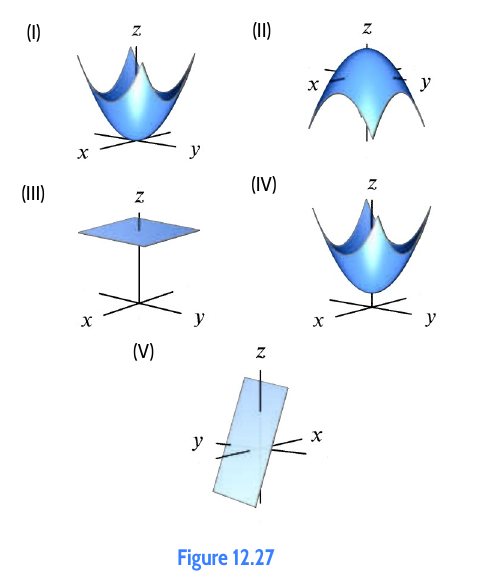
\includegraphics[width=.58\linewidth]{graphs/source-12-2-5.png}\end{center}
\paragraph{Necessary work.} Use \hyperref[transform]{graph transformations}: (a) has an upward vertex above the origin; (b) opens downward; (c) has its upward vertex at the origin; (d) is a tilted plane; (e) is horizontal.
\paragraph{Answer.} (a) IV; (b) II; (c) I; (d) V; (e) III.

\subsection{12.2, Exercise 7: read cross-sections}
\paragraph{Question.} Figure 12.29 shows the graph of $z=f(x,y)$.
\begin{enumerate}
\item[(a)] Suppose $y$ is fixed and positive. Does $z$ increase or decrease as $x$ increases? Graph $z$ against $x$.
\item[(b)] Suppose $x$ is fixed and positive. Does $z$ increase or decrease as $y$ increases? Graph $z$ against $y$.
\end{enumerate}
\begin{center}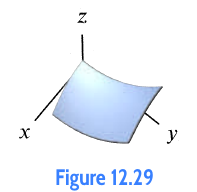
\includegraphics[width=.28\linewidth]{graphs/source-12-2-7.png}\end{center}
\paragraph{Necessary work.} Follow the surface parallel to the indicated input axis; keep the other input fixed. See \hyperref[cross]{cross-sections}. The perspective drawing must be read using its labelled axes.
\paragraph{Answer.} (a) $z$ decreases as $x$ increases; the pictured section bends downward. (b) $z$ increases as $y$ increases; the pictured section bends upward. The following sketches convey shape, not numerical data.
\begin{center}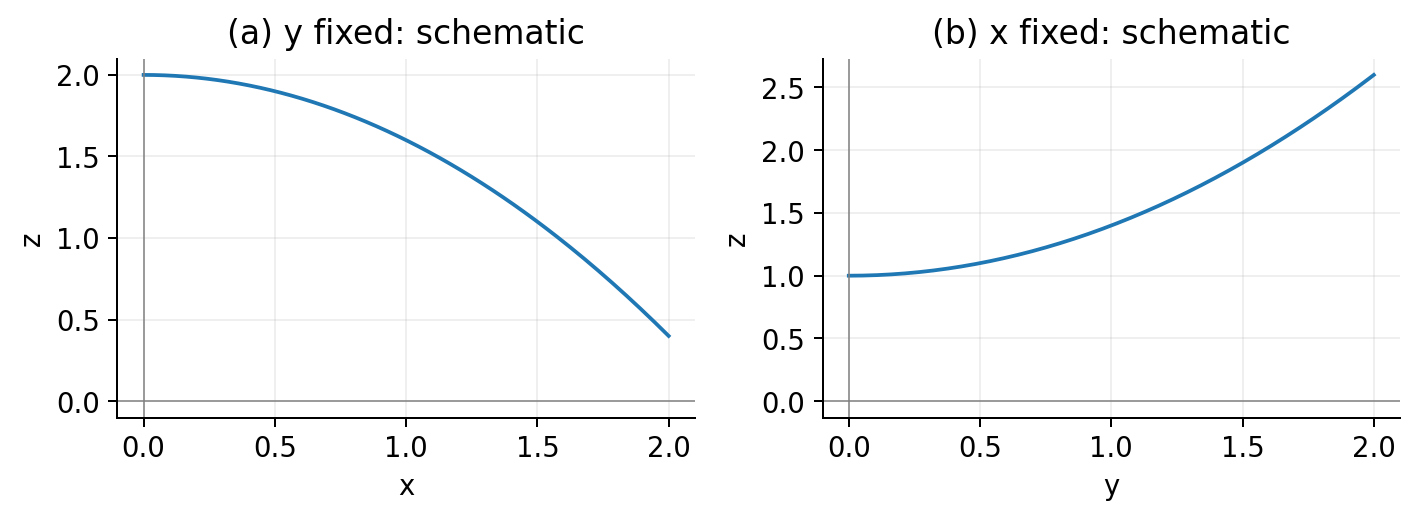
\includegraphics[width=.88\linewidth]{graphs/answer-12-2-7.png}\end{center}

\subsection{12.2, Exercise 9: sphere}
\paragraph{Question.} Sketch a graph of the surface and briefly describe it in words: $x^2+y^2+z^2=9$.
\paragraph{Necessary work.} The sum of squared distances from the origin is $3^2$. Coordinate-plane traces are circles of radius $3$. See \hyperref[graph]{surfaces and the vertical-line test}.
\paragraph{Answer.} A sphere centered at $(0,0,0)$ with radius $3$; axis intercepts are $(\pm3,0,0),(0,\pm3,0),(0,0,\pm3)$. The whole sphere is not the graph of one function $z=f(x,y)$. Its sketch appears in the four-panel figure after Exercise 15.

\subsection{12.2, Exercise 11: downward paraboloid}
\paragraph{Question.} Sketch a graph of the surface and briefly describe it in words: $z=5-x^2-y^2$.
\paragraph{Necessary work.} Reflect $x^2+y^2$ vertically and translate upward by $5$; see \hyperref[transform]{transformations}. Vertical traces are downward parabolas, and horizontal traces satisfy $x^2+y^2=5-c$.
\paragraph{Answer.} A downward-opening circular paraboloid with vertex $(0,0,5)$ and vertical axis. Its intersection with $z=0$ is the circle of radius $\sqrt5$. See the sketch after Exercise 15.

\subsection{12.2, Exercise 13: plane}
\paragraph{Question.} Sketch a graph of the surface and briefly describe it in words: $2x+4y+3z=12$.
\paragraph{Necessary work.} Set two coordinates to zero in turn. Equivalently, $x/6+y/3+z/4=1$. See \hyperref[plane]{planes}.
\paragraph{Answer.} A plane with intercepts $(6,0,0),(0,3,0),(0,0,4)$, or $z=4-\frac23x-\frac43y$. The triangular first-octant patch in the figure is part of an infinite plane.

\subsection{12.2, Exercise 15: cylinder}
\paragraph{Question.} Sketch a graph of the surface and briefly describe it in words: $x^2+z^2=4$.
\paragraph{Necessary work.} Each plane $y=b$ cuts the same circle of radius $2$ in $xz$ coordinates. The missing variable is $y$; see \hyperref[cylinder]{cylinders}.
\paragraph{Answer.} A circular cylinder of radius $2$, centered on and extending in both directions along the $y$-axis. The whole cylinder is not a graph $z=f(x,y)$.
\begin{center}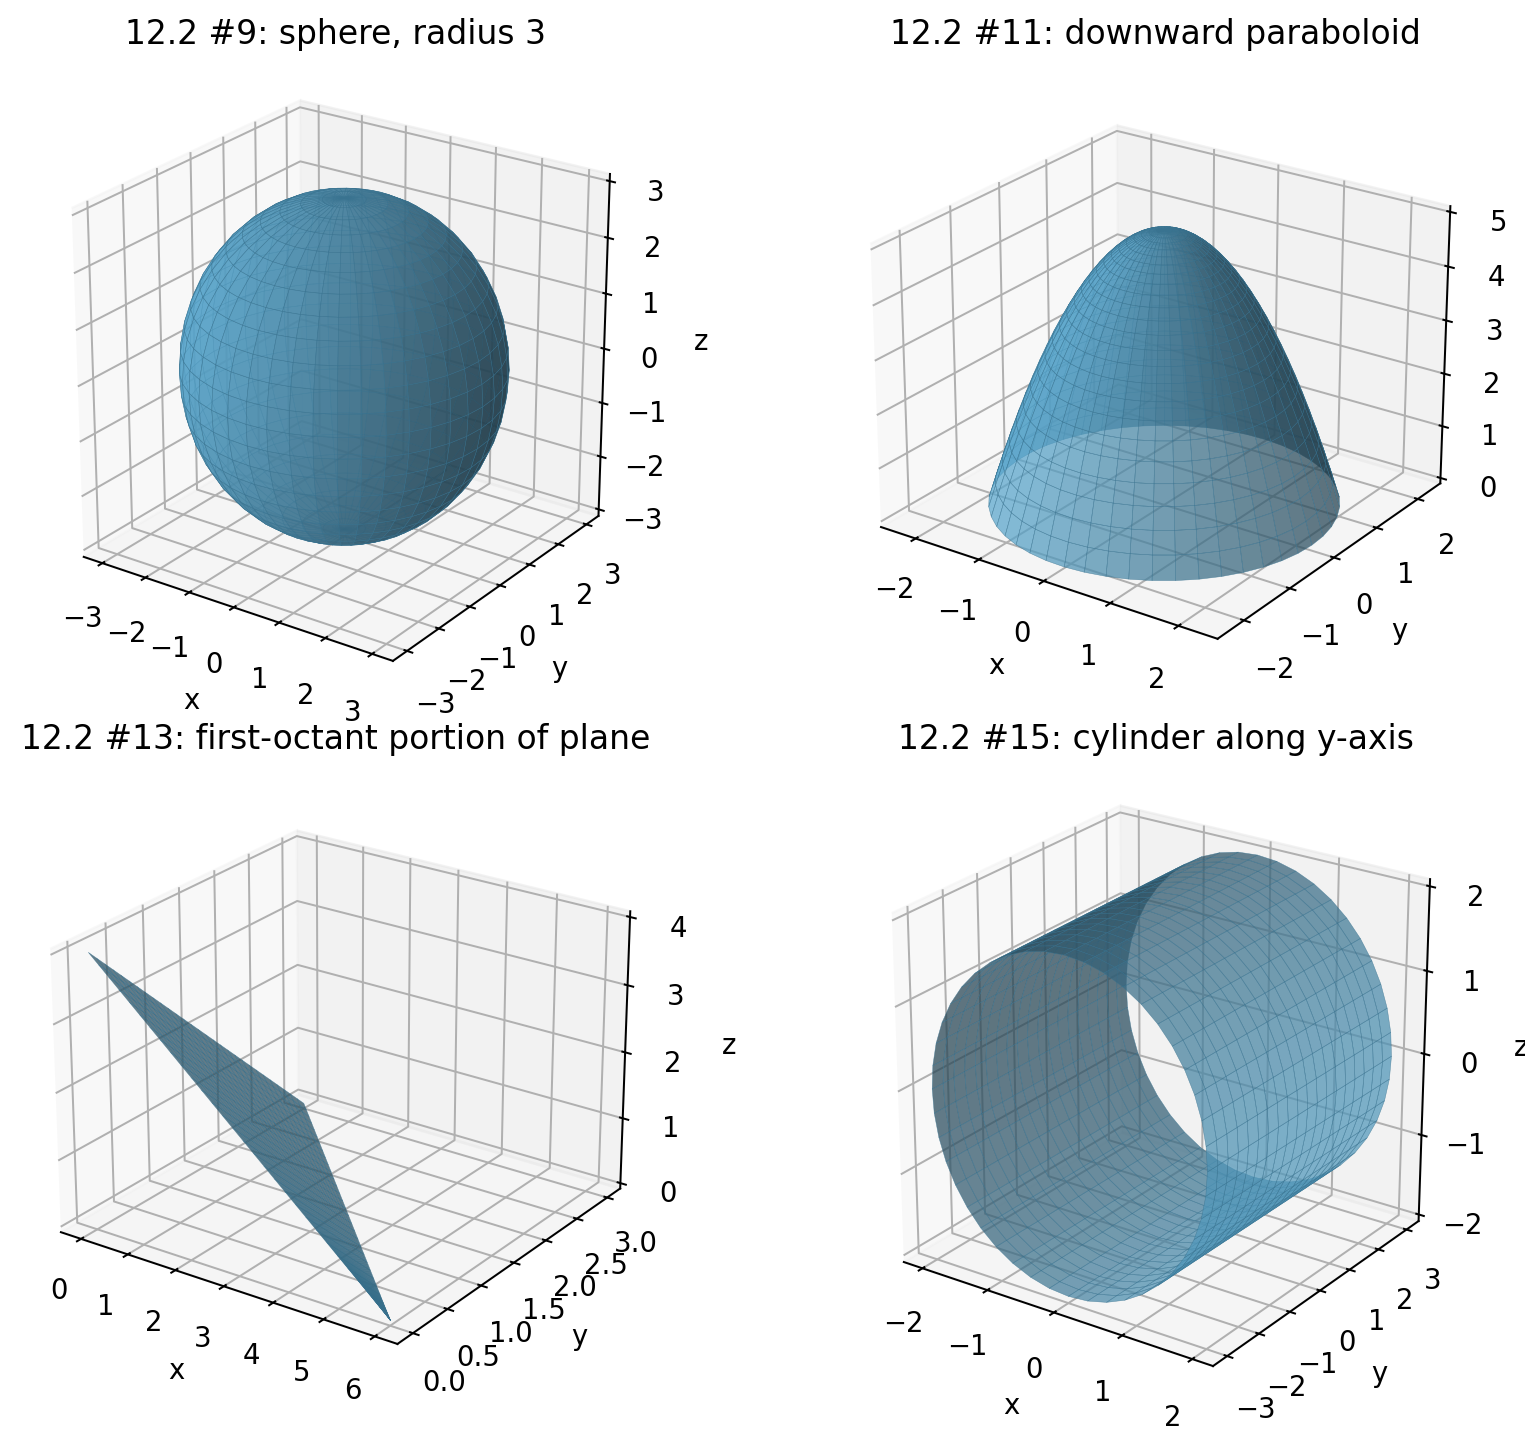
\includegraphics[width=.96\linewidth]{graphs/answer-12-2-surfaces.png}\end{center}

\subsection{12.2, Exercise 17: translate a sphere}
\paragraph{Question.} Find the equation of the surface: a sphere of radius $3$ centered at $(0,\sqrt7,0)$.
\paragraph{Necessary work.} The distance from $(x,y,z)$ to the given center is $3$; square the distance equation. See \hyperref[graph]{surface equations}.
\paragraph{Answer.} $\boxed{x^2+(y-\sqrt7)^2+z^2=9}$.

\subsection{12.2, Exercise 21: drug concentration}
\paragraph{Question.} The concentration $C$, in mg/liter, of a drug in the blood is a function of $x$, the amount in mg of the drug given, and $t$, the time in hours since injection. For $0\le x\le4$ and $t\ge0$,
\[C=f(x,t)=te^{-t(5-x)}.\]
Graph the following single-variable functions and explain their significance in terms of drug concentration: (a) $f(4,t)$; (b) $f(x,1)$.
\paragraph{Necessary work.} Substitute the fixed input, as in \hyperref[cross]{cross-sections}:
\[
f(4,t)=te^{-t}\quad(t\ge0),\qquad f(x,1)=e^{x-5}\quad(0\le x\le4).
\]
For (a), $\frac{d}{dt}(te^{-t})=e^{-t}(1-t)$, so the maximum is $1/e$ at $t=1$. For (b), the exponential is increasing and convex.
\paragraph{Answer.} (a) After a $4$ mg injection, concentration starts at $0$, peaks at $1/e\approx0.368$ mg/liter after $1$ hour, then approaches $0$. (b) One hour after injection, concentration increases from $e^{-5}$ to $e^{-1}$ mg/liter as dose increases from $0$ to $4$ mg. These are interpretations of the stated mathematical model.
\begin{center}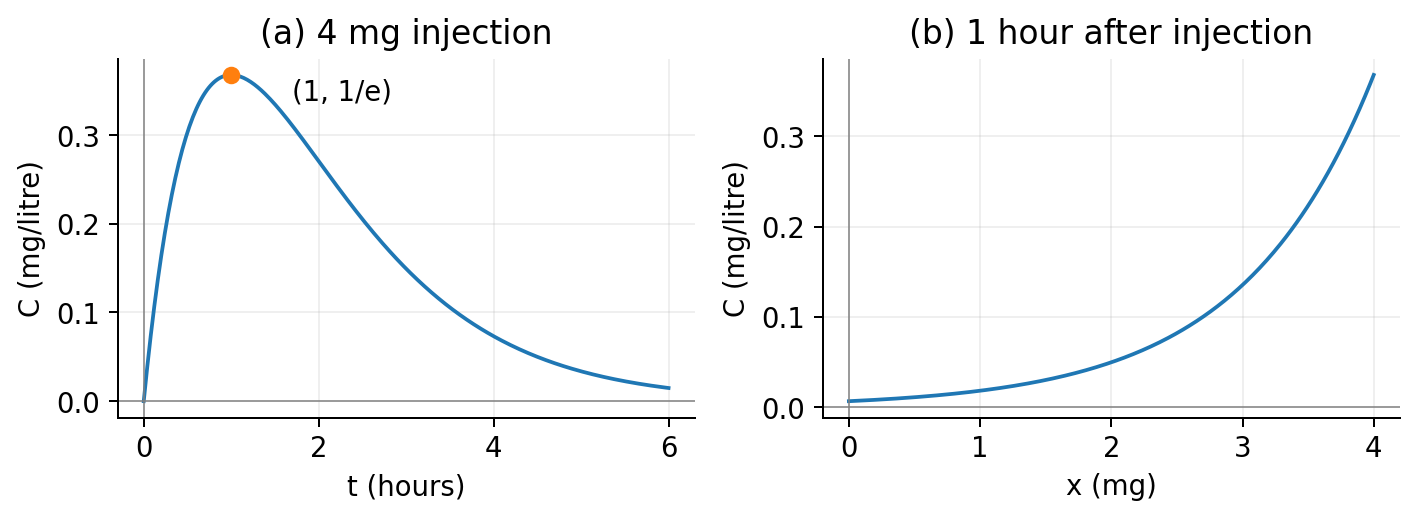
\includegraphics[width=.9\linewidth]{graphs/answer-12-2-21.png}\end{center}

\subsection{12.2, Exercise 27: identify the fixed variable}
\paragraph{Question.} Without a calculator or computer, for $z=x^2+2xy^2$, determine which of (I)--(II) in Figure 12.30 are cross-sections with $x$ fixed and which are cross-sections with $y$ fixed.
\begin{center}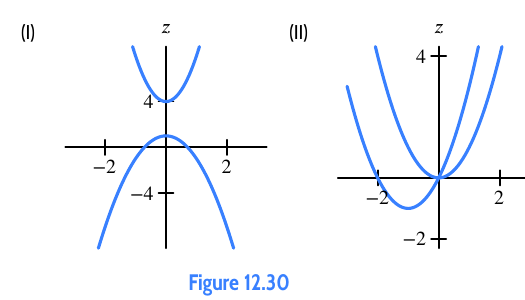
\includegraphics[width=.72\linewidth]{graphs/source-12-2-27.png}\end{center}
\paragraph{Necessary work.} With $x=a$, $z=a^2+2ay^2$: parabolas are symmetric about $y=0$, opening upward for $a>0$ and downward for $a<0$. With $y=b$, $z=x^2+2b^2x=(x+b^2)^2-b^4$: all open upward, pass through $(0,0)$, and have vertices $(-b^2,-b^4)$. See \hyperref[cross]{cross-section families}.
\paragraph{Answer.} I has $x$ fixed; II has $y$ fixed.

\subsection{12.2, Exercise 31: match cross-section families}
\paragraph{Question.} Without a calculator or computer, match the functions with their cross-sections with $x$ fixed in Figure 12.31:
\[
\begin{array}{ll}
\text{(a) }z=1/(1+x^2+y^2),&\text{(b) }z=1+x+y,\\
\text{(c) }z=e^{-x+y},&\text{(d) }z=e^{x-y},\\
\text{(e) }z=\sin(xy),&\text{(f) }z=x^2.
\end{array}
\]
\begin{center}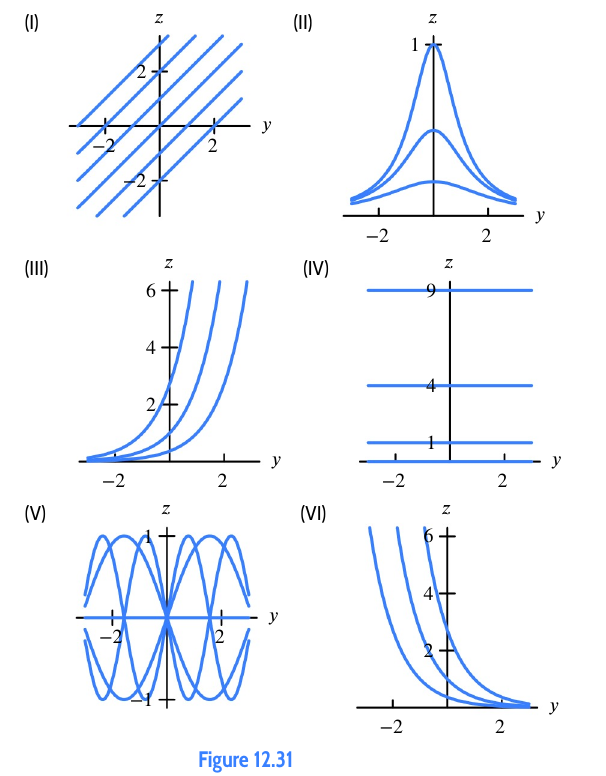
\includegraphics[width=.73\linewidth]{graphs/source-12-2-31.png}\end{center}
\paragraph{Necessary work.} Set $x=a$; see \hyperref[cross]{cross-sections}. The families are, respectively: positive symmetric humps $1/(1+a^2+y^2)$; lines of slope $1$; increasing exponentials $e^{-a}e^y$; decreasing exponentials $e^ae^{-y}$; sines of variable frequency $\sin(ay)$; horizontal lines $z=a^2$.
\paragraph{Answer.} (a) II; (b) I; (c) III; (d) VI; (e) V; (f) IV.

\subsection{12.2, Exercise 41: travelling wave}
\paragraph{Question.} A wave travels along a canal. Let $x$ be the distance along the canal, $t$ be the time, and $z$ be the height of the water above the equilibrium level. The graph of $z$ as a function of $x$ and $t$ is in Figure 12.33.
\begin{enumerate}
\item[(a)] Draw the profile of the wave for $t=-1,0,1,2$. (Put the $x$-axis to the right and the $z$-axis vertical.)
\item[(b)] Is the wave traveling in the direction of increasing or decreasing $x$?
\item[(c)] Sketch a surface representing a wave traveling in the opposite direction.
\end{enumerate}
\begin{center}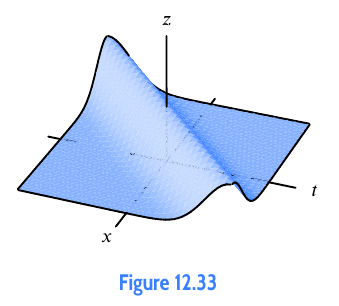
\includegraphics[width=.48\linewidth]{graphs/source-12-2-41.png}\end{center}
\paragraph{Necessary work.} Use \hyperref[cross]{cross-sections} with time fixed. Follow the ridge as $t$ increases: the crest moves toward larger $x$. A schematic translating pulse has the form $z=g(x-vt)$ with $v>0$; reversing time gives $g(x+vt)$. The diagram provides no numerical speed or precise formula.
\paragraph{Answer.} (a) The four hump-shaped profiles shift right as time increases, as sketched below. (b) Increasing $x$. (c) Reverse the ridge direction; the second sketch uses $g(s)=e^{-s^2}$ purely to illustrate a wave moving toward decreasing $x$.
\begin{center}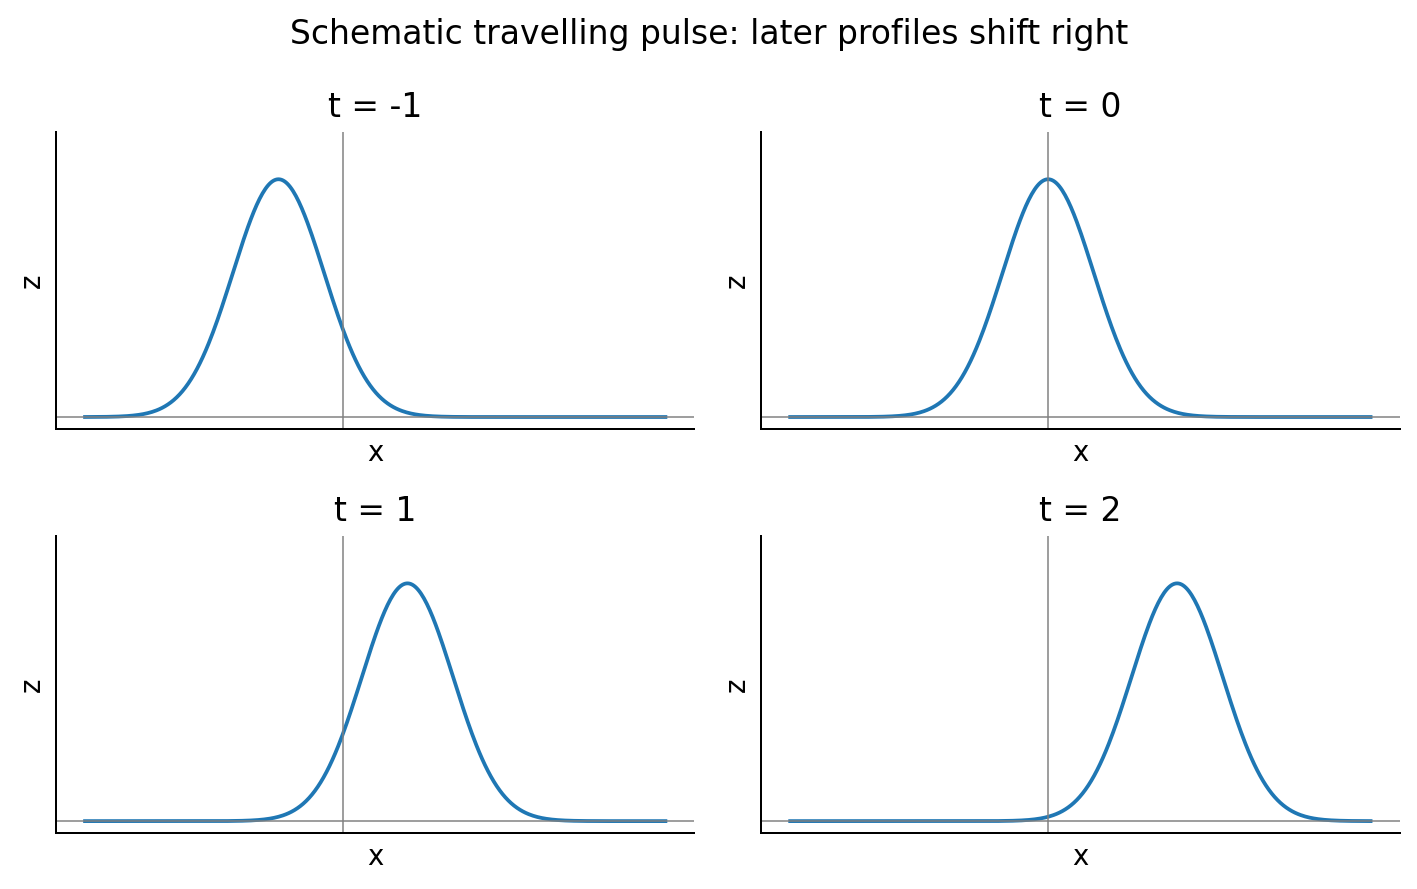
\includegraphics[width=.88\linewidth]{graphs/answer-12-2-41.png}\end{center}
\begin{center}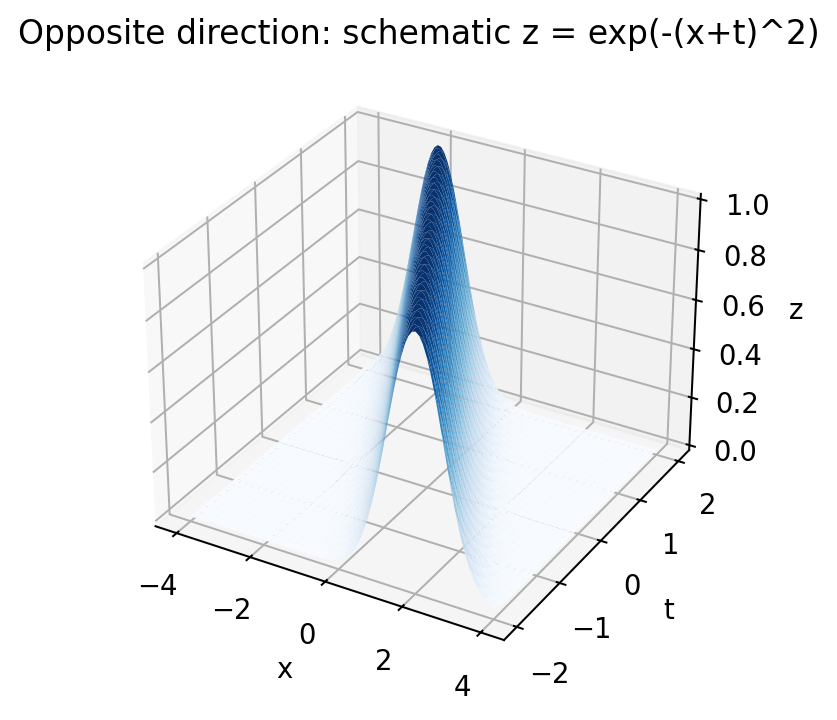
\includegraphics[width=.62\linewidth]{graphs/answer-12-2-41c.png}\end{center}

\section{Suggested textbook practice: Section 12.3}
The following 13 exercises complete the supplied suggested-exercise list. All contour values shown on solution figures are function values, rather than radii.

\subsection{12.3, Exercise 1: surface to contours}
\paragraph{Question.} Sketch a possible contour diagram for the surface below, marked with reasonable $z$-values. (Note: There are many possible answers.)
\begin{center}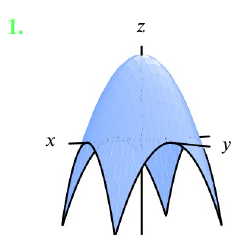
\includegraphics[width=.35\linewidth]{graphs/source-12-3-1.png}\end{center}
\paragraph{Necessary work.} The surface is a downward bowl. Horizontal slices project to concentric circles, with larger heights nearer the center; see \hyperref[contour]{contours}. One model consistent with its shape is $z=4-x^2-y^2$.
\paragraph{Answer.} A valid diagram has center value $4$ and circles $x^2+y^2=4-c$ labelled $c=3,2,1,0$ from inside outward. The particular heights are a reasonable choice, not measurements from the source.
\begin{center}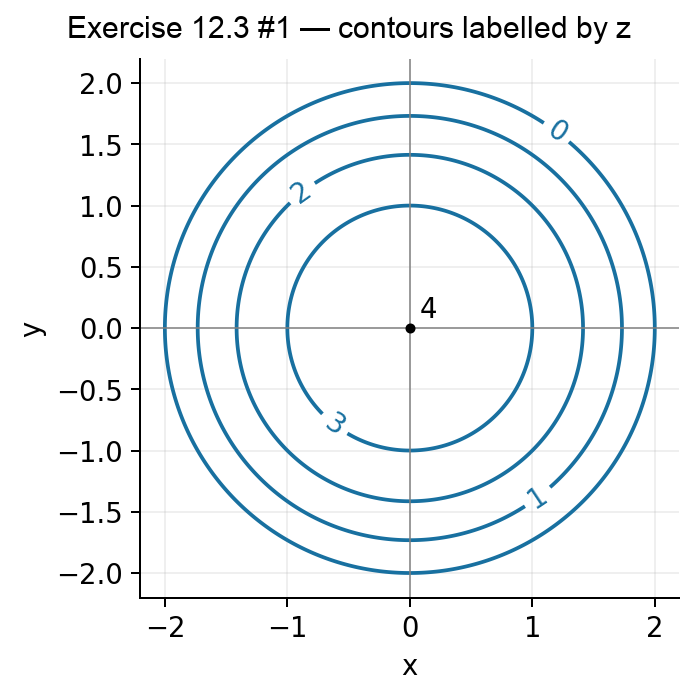
\includegraphics[width=.51\linewidth]{graphs/answer-12-3-1.png}\end{center}

\subsection{12.3, Exercise 3: a circular depression}
\paragraph{Question.} Sketch a possible contour diagram for the surface below, marked with reasonable $z$-values. (Note: There are many possible answers.)
\begin{center}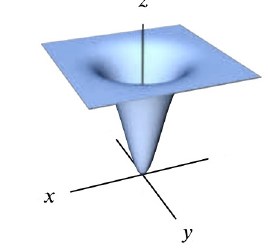
\includegraphics[width=.36\linewidth]{graphs/source-12-3-3.png}\end{center}
\paragraph{Necessary work.} The center is low and the surface rises outward while flattening. Thus choose concentric circles whose values increase outward; see \hyperref[contour]{contour interpretation}. For a concrete illustration, $z=4(1-e^{-(x^2+y^2)})$ has this qualitative shape. Its level $c$ has radius $\sqrt{-\ln(1-c/4)}$, for $0<c<4$.
\paragraph{Answer.} The labelled circles below give one possible answer. Their labels increase from $1$ through $2,3,3.5$; the center has height $0$ in this illustrative model. Other reasonable numerical choices are valid. These levels are not equally spaced, so do not compare their gaps as if their height increments were equal.
\begin{center}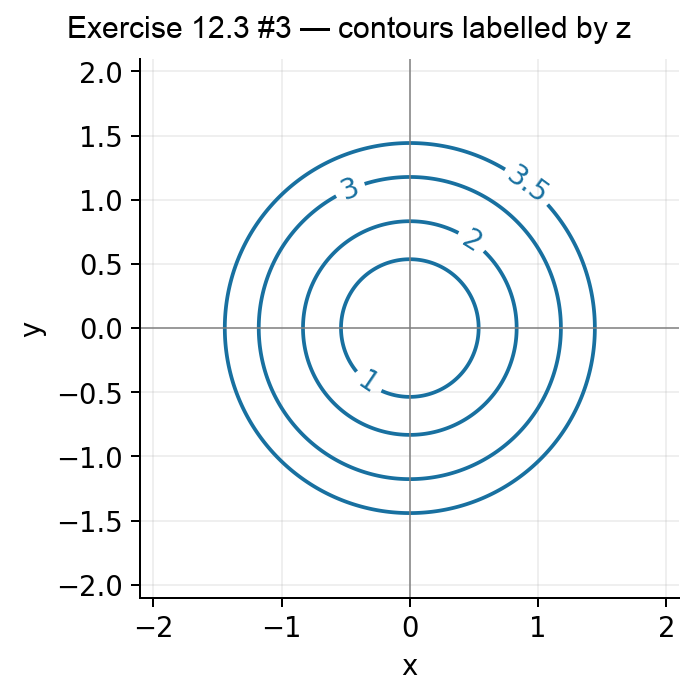
\includegraphics[width=.51\linewidth]{graphs/answer-12-3-3.png}\end{center}

\subsection{12.3, Exercise 5: read a contour value}
\paragraph{Question.} Use the contour diagram of $f(x,y)$ given in Figure 12.52 to find $f(1,3)$.
\begin{center}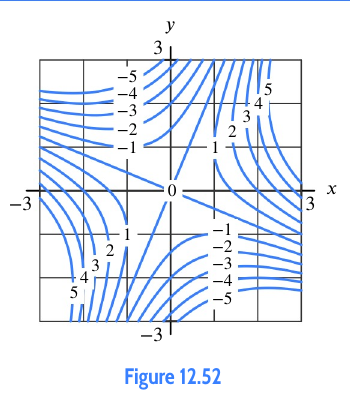
\includegraphics[width=.53\linewidth]{graphs/source-12-3-5.png}\end{center}
\paragraph{Necessary work.} Locate $(1,3)$ and follow its curve to the label $-1$; see \hyperref[estimate]{reading contour values}. Do not confuse the nearby sloping zero contour with the curve through this point.
\paragraph{Answer.} $\boxed{f(1,3)=-1}$.

\subsection{12.3, Exercise 7: find a point on a level set}
\paragraph{Question.} Use the contour diagram of $f(x,y)$ given in Figure 12.52 to find a point where $f(x,y)=0$.
\begin{center}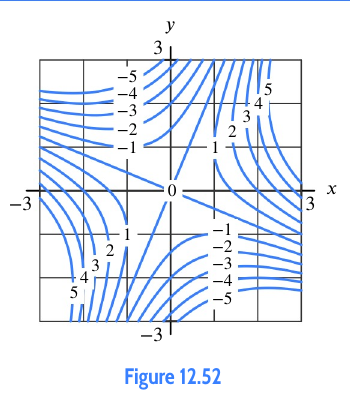
\includegraphics[width=.45\linewidth]{graphs/source-12-3-5.png}\end{center}
\paragraph{Necessary work.} Choose a point on a contour labelled $0$; see \hyperref[contour]{level sets}. The origin lies on that level set.
\paragraph{Answer.} $(0,0)$; other points on the zero contour are also valid.

\subsection{12.3, Exercise 9: contour through a point}
\paragraph{Question.} Let $f(x,y)=3x^2y+7x+20$. Find an equation for the contour that goes through the point $(5,10)$.
\paragraph{Necessary work.} First find the output at the point: $f(5,10)=3(25)(10)+35+20=805$. Then set the function equal to that value; see \hyperref[contour]{finding contours algebraically}.
\paragraph{Answer.} $\boxed{3x^2y+7x+20=805}$. Equivalently $y=(785-7x)/(3x^2)$, with $x\ne0$.

\subsection{12.3, Exercise 11: match surfaces and contour diagrams}
\paragraph{Question.} Match the surfaces (a)--(e) in Figure 12.53 with the contour diagrams (I)--(V) in Figure 12.54.
\begin{center}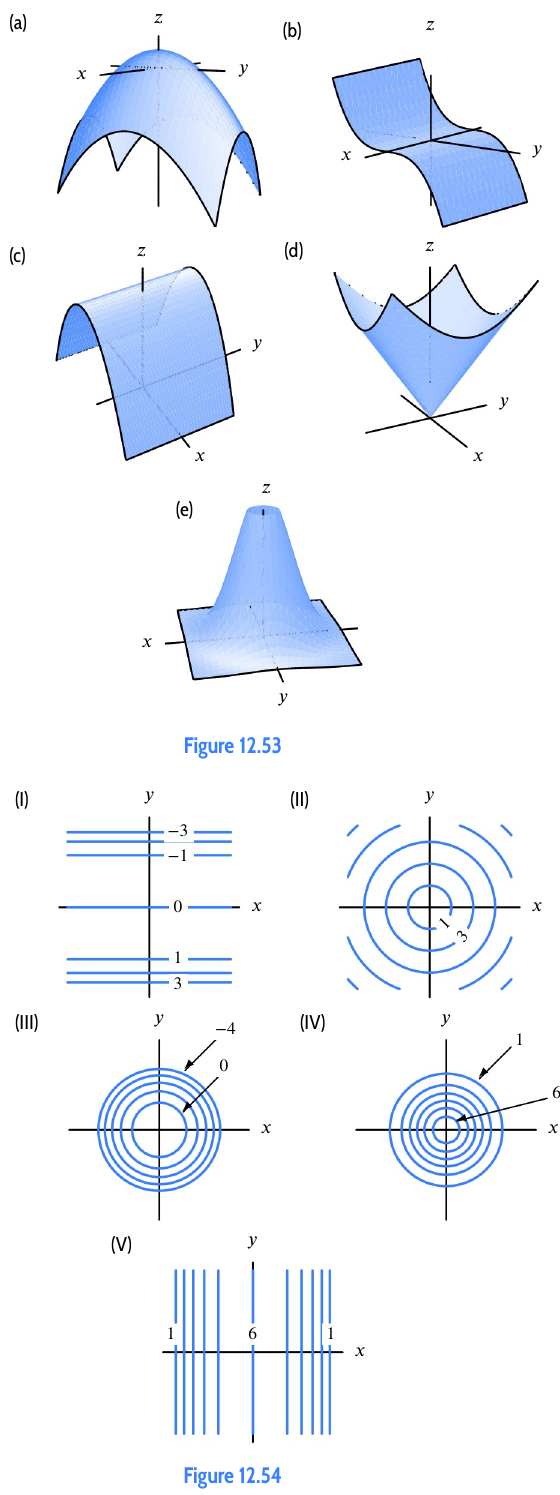
\includegraphics[height=.70\textheight,keepaspectratio]{graphs/source-12-3-11.png}\end{center}
\paragraph{Necessary work.} Use both shape and labels; see \hyperref[contour]{contour interpretation}. Surface (a) is a downward radial bowl. Surface (b) is a trough: its height is smallest on the central line and rises in either $y$ direction, producing paired horizontal contours. Surface (c) is a downward parabolic cylinder with a maximum along its central ridge and no change parallel to $y$, producing paired vertical contours. Surface (d) is an upward cone; (e) is a high central radial mound.
\paragraph{Answer.} (a) III (circle values decrease outward); (b) I (horizontal lines with values decreasing as $y$ increases); (c) V (vertical paired lines); (d) II (evenly spaced circles); (e) IV (circle values highest near the center).

\subsection{12.3, Exercise 13: tables to contour diagrams}
\paragraph{Question.} Match Tables 12.6--12.9 with contour diagrams (I)--(IV) in Figure 12.56. The four tables and all four candidate diagrams are reproduced here.
\begin{center}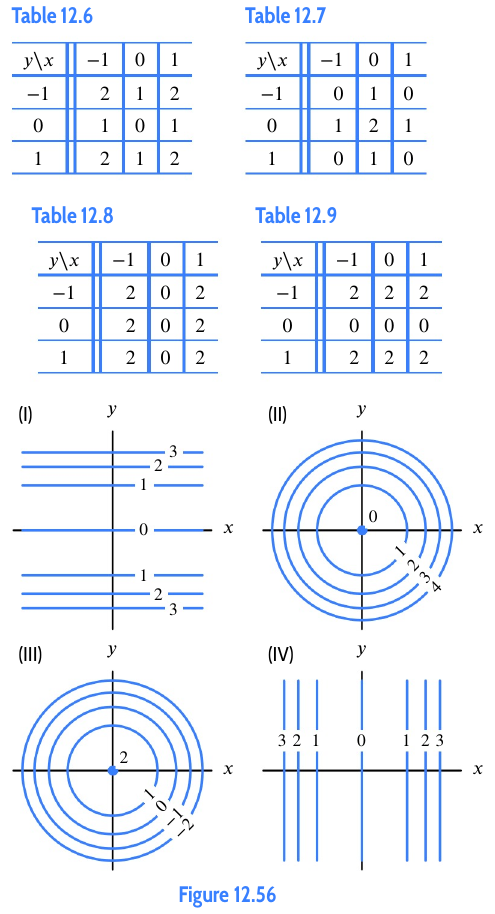
\includegraphics[width=.62\linewidth]{graphs/source-12-3-13.png}\end{center}
\paragraph{Necessary work.} See \hyperref[table]{tables and contours}. Table 12.6 has a central minimum, consistent with $x^2+y^2$. Table 12.7 has a central maximum, consistent with $2-x^2-y^2$. In Table 12.8 the entries depend only on $x$; in Table 12.9 they depend only on $y$. The corresponding vertical or horizontal lines must also have the matching labels. These simple formulas explain the matches; a finite table alone does not uniquely determine a function everywhere.
\paragraph{Answer.} Table 12.6 $\to$ II; Table 12.7 $\to$ III; Table 12.8 $\to$ IV; Table 12.9 $\to$ I.

\subsection{12.3, Exercise 15: parallel line contours}
\paragraph{Question.} Sketch a contour diagram for $f(x,y)=3x+3y$ with at least four labeled contours. Describe in words the contours and how they are spaced.
\paragraph{Necessary work.} Set $3x+3y=c$, giving $y=-x+c/3$; see \hyperref[contour]{algebraic contours}. Choose, for example, $c=-6,-3,0,3,6$.
\paragraph{Answer.} Parallel lines of slope $-1$, equally spaced for equally spaced values of $c$. A level change $\Delta c$ gives perpendicular separation $|\Delta c|/(3\sqrt2)$; for $\Delta c=3$, this is $1/\sqrt2$.
\begin{center}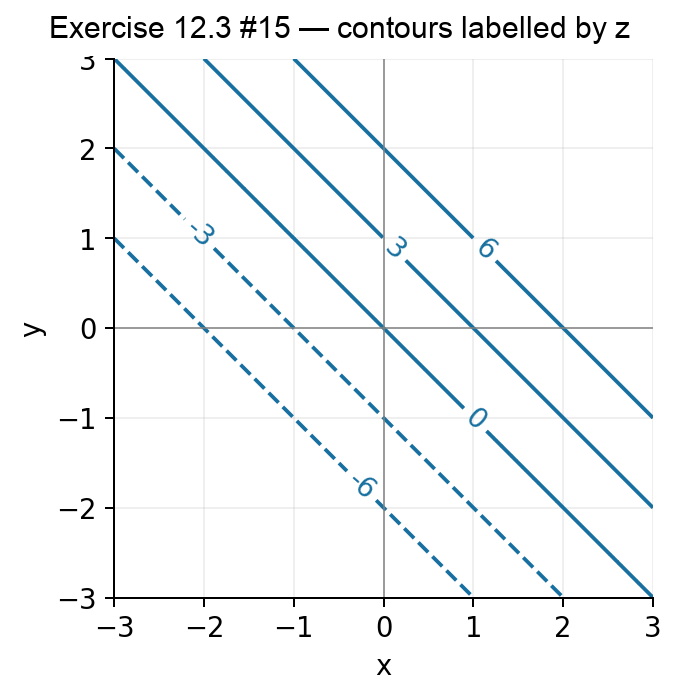
\includegraphics[width=.51\linewidth]{graphs/answer-12-3-15.png}\end{center}

\subsection{12.3, Exercise 17: downward bowl contours}
\paragraph{Question.} Sketch a contour diagram for $f(x,y)=-x^2-y^2+1$ with at least four labeled contours. Describe in words the contours and how they are spaced.
\paragraph{Necessary work.} The level equation is $x^2+y^2=1-c$. Levels exist only for $c\le1$; see \hyperref[contour]{circular contours}. Use $c=0,-1,-2,-3$, whose radii are $1,\sqrt2,\sqrt3,2$.
\paragraph{Answer.} Concentric circles centered at the origin, with decreasing labels outward. For equal decreases in $c$, successive circles get closer together farther from the center, indicating increasing steepness. The $c=1$ level is the origin alone.
\begin{center}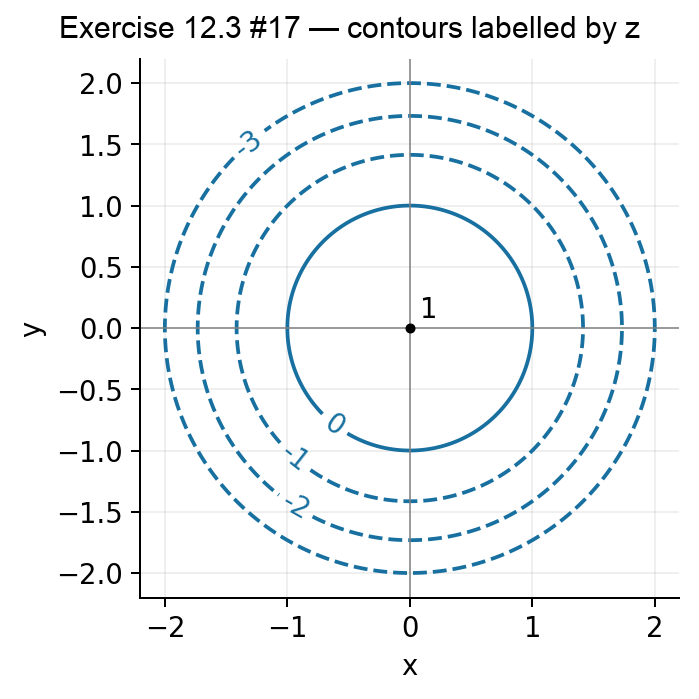
\includegraphics[width=.51\linewidth]{graphs/answer-12-3-17.png}\end{center}

\subsection{12.3, Exercise 19: parabolic contours}
\paragraph{Question.} Sketch a contour diagram for $f(x,y)=y-x^2$ with at least four labeled contours. Describe in words the contours and how they are spaced.
\paragraph{Necessary work.} Set $y-x^2=c$, so $y=x^2+c$. Choose $c=-2,-1,0,1,2$; see \hyperref[contour]{algebraic contours}.
\paragraph{Answer.} Upward-opening parabolas with vertices $(0,c)$, translated vertically. For equal increments of $c$, the vertical separation at fixed $x$ is constant. Their perpendicular separation is not constant; the curves become closer in the transverse direction as $|x|$ grows.
\begin{center}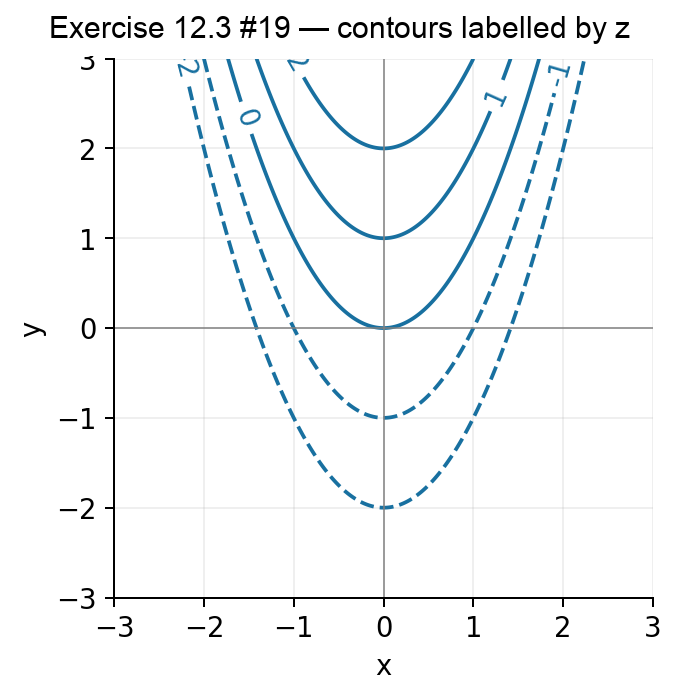
\includegraphics[width=.51\linewidth]{graphs/answer-12-3-19.png}\end{center}

\subsection{12.3, Exercise 25: interpret contour labels}
\paragraph{Question.} Each contour diagram (a)--(c) in Figure 12.59 shows satisfaction with quantities of two items $X$ and $Y$ combined. Match (a)--(c) with the items in (I)--(III):
\begin{enumerate}
\item[(I)] $X$: Income; $Y$: Leisure time.
\item[(II)] $X$: Income; $Y$: Hours worked.
\item[(III)] $X$: Hours worked; $Y$: Time spent commuting.
\end{enumerate}
\begin{center}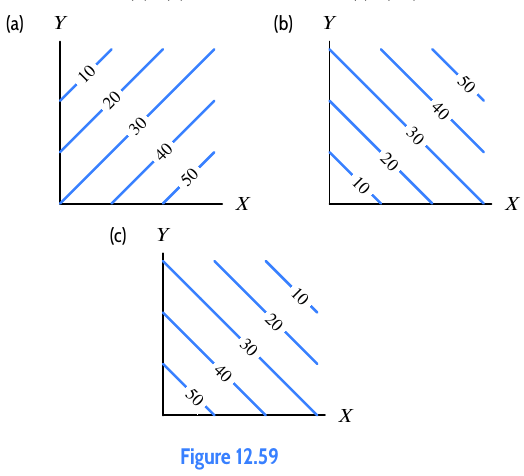
\includegraphics[width=.67\linewidth]{graphs/source-12-3-25.png}\end{center}
\paragraph{Necessary work.} Track whether the labels increase or decrease on moving right and upward; see \hyperref[estimate]{reading contour diagrams}. In (a), increasing $X$ raises satisfaction but increasing $Y$ lowers it. In (b), increasing either quantity raises satisfaction. In (c), increasing either quantity lowers satisfaction. Use the preferences represented by this question's model.
\paragraph{Answer.} (a) II; (b) I; (c) III.

\subsection{12.3, Exercise 27: trade-off along a contour}
\paragraph{Question.} Figure 12.61 shows a contour diagram of Dan's happiness with snacks of different numbers of cherries and grapes. (a) What is the slope of the contours? (b) What does the slope tell you?
\begin{center}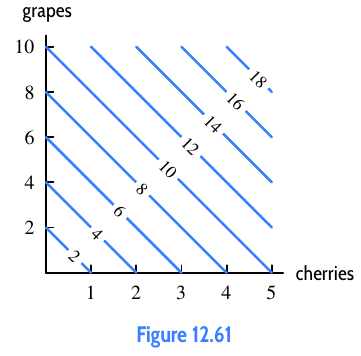
\includegraphics[width=.50\linewidth]{graphs/source-12-3-27.png}\end{center}
\paragraph{Necessary work.} On a fixed contour, increasing cherries by $1$ decreases grapes by $2$. Thus
\[\frac{\Delta(\text{grapes})}{\Delta(\text{cherries})}=-2.\]
See \hyperref[contour]{constant-output trade-offs}.
\paragraph{Answer.} (a) $-2$ grapes per cherry. (b) Replacing two grapes with one cherry leaves Dan's happiness unchanged in this model; conversely, he needs two additional grapes to compensate for one fewer cherry.

\subsection{12.3, Exercise 47: profit contours}
\paragraph{Question.} A manufacturer sells two goods, one at a price of \$3000 a unit and the other at a price of \$12,000 a unit. A quantity $q_1$ of the first good and $q_2$ of the second good are sold at a total cost of \$4000 to the manufacturer.
\begin{enumerate}
\item[(a)] Express the manufacturer's profit, $\pi$, as a function of $q_1$ and $q_2$.
\item[(b)] Sketch curves of constant profit in the $q_1q_2$-plane for $\pi=10{,}000$, $\pi=20{,}000$, and $\pi=30{,}000$, and the break-even curve $\pi=0$.
\end{enumerate}
\paragraph{Necessary work.} Revenue minus total cost gives profit in dollars. Then set profit to a constant $c$, as in \hyperref[contour]{level curves}:
\[
\pi(q_1,q_2)=3000q_1+12000q_2-4000,\qquad
q_2=-\frac14q_1+\frac{c+4000}{12000}.
\]
Restrict the economic diagram to $q_1,q_2\ge0$. The intercepts are
\[
\begin{array}{c|cc}
c\text{ (dollars)}&q_1\text{-intercept}&q_2\text{-intercept}\\\hline
0&4/3&1/3\\
10{,}000&14/3&7/6\\
20{,}000&8&2\\
30{,}000&34/3&17/6
\end{array}
\]
\paragraph{Answer.} (a) $\boxed{\pi=3000q_1+12000q_2-4000}$ dollars. (b) The four parallel segments below have slope $-1/4$; profit increases toward the upper right. If quantities must be whole units, only integer points on or between these continuous model contours represent feasible sales.
\begin{center}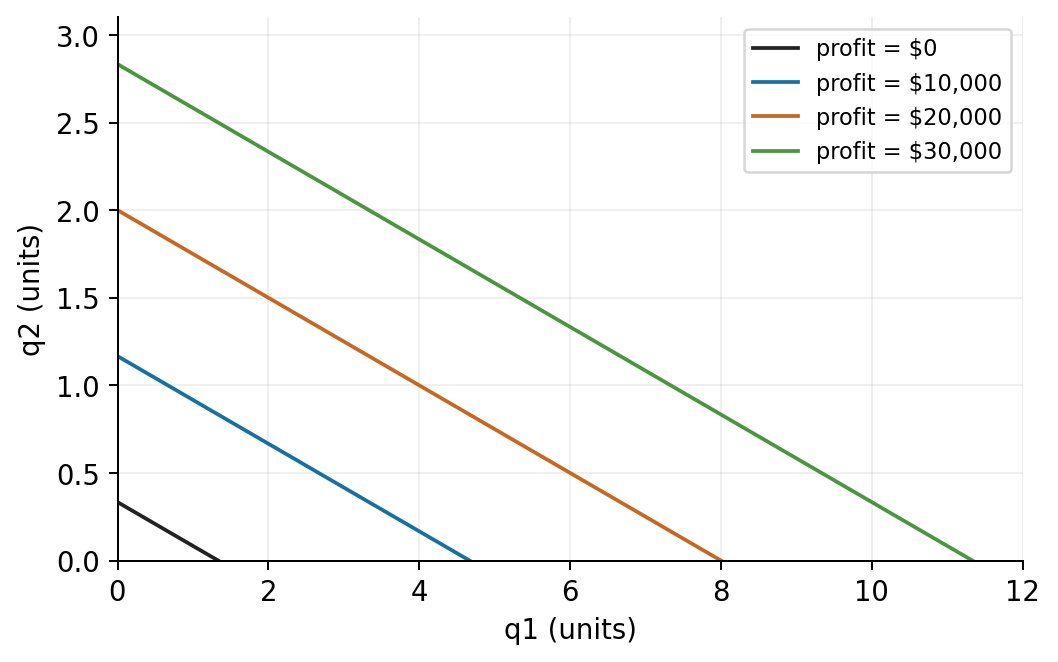
\includegraphics[width=.74\linewidth]{graphs/answer-12-3-47.png}\end{center}

\section{Original self-test}\label{selftest}
These questions are newly written and independent of the textbook exercise bank. Try them without reading the answers that follow. Their figures and tables contain all data needed.
\subsection*{Questions}
\begin{enumerate}[label=\textbf{Q\arabic*.},leftmargin=*]
\item A set in $\R^3$ is given by $x^2+y^2+z^2=9$. Is the whole set a graph $z=f(x,y)$? Explain using one input pair. State a suitable domain for each branch after splitting it into two graphs. (See \hyperref[surface]{surface description}.)
\item Describe $z=3-2x+y$: object, axis intercepts, $x=0$ and $y=0$ traces, directions of increase, and infinite or finite extent. (See \hyperref[surface]{surfaces}.)
\item For $z=x^2-y^2$, find the two sections $x=2$ and $y=-1$ and identify each graph's shape and plane. (See \hyperref[cross]{cross-sections}.)
\item For $F(x,y)=y^2+2xy$, write the $x=0$, $x=1$, $y=0$, and $y=2$ cross-sections. State the horizontal plotting coordinate of each family. (See \hyperref[cross]{cross-sections}.)
\item In $\R^3$, describe $y^2+z^2=4$. Which coordinate is free? Can the full set be written as $z=f(x,y)$? (See \hyperref[cylinder]{cylinders}.)
\item For $f=x^2+4y^2$, find and sketch the $c=0,4,16$ contours with axis intercepts and allowable $c$. What is the 3D shape? (See \hyperref[radial]{algebraic contours}.)
\item For $g(x,y)=9-\sqrt{x^2+y^2}$, give $g=8,7,6$ contour radii and tell where the values increase. (See \hyperref[radial]{contours}.)
\item For $p(x,y)=3x-y+2$, write the $p=-1,2,5$ contours, their common slope, and a direction of increasing values. (See \hyperref[plane]{linear contours}.)
\item Read the table below, with $x$ across columns, $y$ down rows, and entries $v(x,y)$ in metres. Find $v(2,1)$ exactly. Estimate where $v=5$ crosses rows $y=0,1,2$ by linear interpolation. Sketch the approximate contour inside the table's square. (See \hyperref[table]{table construction}.)
\begin{center}\begin{tabular}{c|rrr}\toprule $y\backslash x$ (m)&0&1&2\\\midrule0&9&7&5\\1&8&6&4\\2&7&5&3\\\bottomrule\end{tabular}\end{center}
\item Use the following labelled contour map of $q(x,y)=12-x^2-y^2$. The point $A=(1.5,0)$ lies between the contours $10$ and $8$. Give a range for $q(A)$, estimate it from the map, then compute it exactly from the formula. What do close equal-label-interval contours imply? (See \hyperref[estimate]{map reading}.)\fig{.78}{10-self-test.png}
\item For $s(x,y)=x^2-y^2$, describe the $s=0$, $s=3$, and $s=-3$ levels. How many components does each have? Can distinct-value contours cross? (See \hyperref[saddle]{saddle contours}.)
\item A triangular tent spans $0\leq x\leq4$ m and $0\leq y\leq2$ m; its ridge is along $x=2$ at height $6$ m, and its side edges have height $0$. Find its roof-height formula and the $3$ m contour. (See \hyperref[tent]{finite-domain roof}.)
\item (Supplementary) Starting from $z=x^2+y^2$, describe $z=(x+2)^2+(y-1)^2-3$ and name its vertex. (See \hyperref[transform]{transformations}.)
\item (Supplementary) A production model is $P(N,V)=\sqrt{NV}$ for positive $N,V$. Find the $P=4$ contour and interpret how $V$ must change if $N$ doubles. (See \hyperref[supplement]{production}.)
\item (Preview) If $H(x,y,z)=x^2+y^2+z^2$, describe the level surfaces $H=0,1,4$. If $J=z-y$, describe $J=2$. State which objects are spheres and which are planes. (See \hyperref[preview]{level surfaces}.)
\end{enumerate}
\subsection*{Answers and correction notes}
\begin{enumerate}[label=\textbf{A\arabic*.},leftmargin=*]
\item No: $(x,y)=(0,0)$ yields $z=\pm3$. The two branches are $z=\pm\sqrt{9-x^2-y^2}$ on $x^2+y^2\leq9$.
\item An infinite plane. Intercepts $(3/2,0,0),(0,-3,0),(0,0,3)$. At $x=0$, $z=3+y$; at $y=0$, $z=3-2x$. Height decreases with increasing $x$ and increases with increasing $y$.
\item $x=2:\ z=4-y^2$ is downward in the plane $x=2$; $y=-1:\ z=x^2-1$ is upward in the plane $y=-1$.
\item $x=0:\ z=y^2$; $x=1:\ z=y^2+2y$ (horizontal axis $y$). $y=0:\ z=0$; $y=2:\ z=4+4x$ (horizontal axis $x$).
\item $x$ is free; the set is a radius-2 circular cylinder parallel to $x$. It is not a full $z$-function because $z=\pm\sqrt{4-y^2}$ at interior values $|y|<2$.
\item $c<0$ empty; $c=0$ origin; $c=4$ ellipse intercepts $(\pm2,0),(0,\pm1)$; $c=16$ ellipse intercepts $(\pm4,0),(0,\pm2)$. The graph is an upward elliptic paraboloid.
\item $g=c$ gives radius $9-c$, hence $1,2,3$. Higher values lie toward the origin, where $g(0,0)=9$.
\item $y=3x+3$, $y=3x$, $y=3x-3$ for $p=-1,2,5$. All slopes are $3$. Move toward $(3,-1)$ to increase $p$.
\item $v(2,1)=4$ m. At $y=0$, $v=5$ at $x=2$; at $y=1$, halfway between $6$ and $4$ gives $x=1.5$; at $y=2$, $v=5$ at $x=1$. Join $(2,0),(1.5,1),(1,2)$. A matching affine interpolation is $2x+y=4$ within the square; it is not established globally.
\item $8<q(A)<10$; radial interpolation gives about $9.7$, while direct substitution gives $9.75$. Close contours for equal differences in $q$ indicate faster horizontal change / a steeper surface.
\item $s=0$ is $y=\pm x$, two intersecting lines that together form one connected set. $s=3$ has two left/right opening branches; $s=-3$ has two up/down opening branches. Different-value contours cannot cross for a function.
\item $h=3x$ for $0\leq x\leq2$ and $h=12-3x$ for $2\leq x\leq4$, with $0\leq y\leq2$. At $h=3$, $x=1$ and $x=3$, each a segment $0\leq y\leq2$.
\item Translation by $(-2,1,-3)$; upward paraboloid with vertex $(-2,1,-3)$.
\item $\sqrt{NV}=4$ gives $NV=16$, hence $V=16/N$. If $N$ doubles, $V$ halves to maintain production $4$.
\item $H=0$ is the single origin; $H=1,4$ are spheres centered at the origin with radii $1,2$. $J=2$ is the infinite plane $z=y+2$, parallel to the $x$-axis.
\end{enumerate}

\section{Coverage and source audit}\label{audit}
\subsection{Scope and provenance}
The six weekly PDFs contain 54 pages. The main requested textbook boundary is section 12.2 (printed pp.~702--711; PDF pp.~722--731) and section 12.3 (printed pp.~711--725; PDF pp.~731--745) of the 8th-edition text. Textbook content after the 12.4 heading on printed p.~725 is excluded. The supplementary preview is drawn from weekly lecture files only. The user supplied 13 suggested exercises from each section; all 26 appear in \hyperref[textbook]{textbook practice}. Graphs in \texttt{graphs/01--10} are original labelled reconstructions generated by \texttt{graphs/generate\_graphs.py}; \texttt{graphs/source-*} are cropped source diagrams from the textbook. The diagrams serve the questions shown beside them. All mathematical content has been checked independently against page images and text extraction.

\subsection{Page-to-topic checklist}
\small
\begin{longtable}{p{.40\linewidth}p{.50\linewidth}}
\toprule Source and page(s) & Covered at\\\midrule\endhead
\texttt{Week2.pdf} p.~1 & \hyperref[surface]{plane surface}, \hyperref[cross]{cross-sections}, weekly page 1\\
\texttt{Week2.pdf} p.~2 & \hyperref[surface]{surface test}, \hyperref[cylinder]{cylinders}, weekly page 2\\
\texttt{Week2.pdf} p.~3 & \hyperref[cross]{six trace family}, weekly page 3\\
\texttt{Week2.pdf} pp.~4--5 & \hyperref[contour]{definitions}, \hyperref[radial]{bowl/cone levels}, weekly pages 4--5\\
\texttt{Week2.pdf} p.~6 & \hyperref[plane]{parallel plane contours}, weekly page 6\\
\texttt{Week2.pdf} pp.~7--8 & \hyperref[saddle]{complete table and saddle contours}, weekly pages 7--8\\
\texttt{Week2.pdf} pp.~9--10 & \hyperref[tent]{finite tent roof}, weekly pages 9--10\\
\texttt{sep+14.pdf} pp.~1--4 & \hyperref[graph]{graph test}, \hyperref[transform]{transformation}, \hyperref[cross]{saddle slices}, weekly source section\\
\texttt{sep+16.pdf} pp.~1--4 & \hyperref[cylinder]{free-variable cylinder}, \hyperref[radial]{downward bowl contours}, weekly source section\\
\texttt{sep+18.pdf} pp.~1--4 & \hyperref[table]{full numeric interpolation table}, \hyperref[saddle]{saddle comparison}, weekly source section\\
\texttt{MAT235H-5201-Sept-16.pdf} pp.~1--6 & \hyperref[supplement]{12.1 recap} and weekly review questions; p.~1 administrative information only\\
Same PDF pp.~7--12 & Complete wind-chill table, coordinate questions, heater cross-sections, plane in \hyperref[weekly]{weekly questions}; \hyperref[cross]{method}\\
Same PDF pp.~13--19 & \hyperref[cylinder]{cylinders}, \hyperref[cross]{traces and upper-hemisphere slice}, weekly discussion\\
Same PDF pp.~20--23 & \hyperref[radial]{contours}, \hyperref[plane]{linear levels}, \hyperref[saddle]{table and saddle}, weekly questions\\
Same PDF pp.~24--27 & \hyperref[preview]{12.4 preview} and \hyperref[weekly]{airline/plane/table/surface questions}\\
\texttt{MAT235H-5201-Sept-17.pdf} pp.~1--3 & \hyperref[preview]{plane/cylinder/sphere preview}, weekly questions\\
Same PDF pp.~4--5 & \hyperref[preview]{12.5 three-input levels}, weekly question and self-test\\
Textbook 12.2 pp.~702--707 & \hyperref[graph]{graphs}, \hyperref[transform]{shifts and bell}, \hyperref[cross]{saddle and plane traces}, \hyperref[cylinder]{cylinder example}\\
Textbook 12.2 pp.~707--711 & All user-listed odd exercises in \hyperref[textbook]{practice}; images where questions require them\\
Textbook 12.3 pp.~711--718 & \hyperref[estimate]{corn map/estimation}, \hyperref[radial]{cone/bowl}, \hyperref[saddle]{saddle table}, \hyperref[supplement]{production}\\
Textbook 12.3 pp.~718--725 & All user-listed odd exercises in \hyperref[textbook]{practice}; images where questions require them\\
\bottomrule\end{longtable}\normalsize

\subsection{Problem-type and exercise checklist}
Every \emph{Problem type} section in this file has a source-labelled complete question, worked solution, separately labelled answer, relevant diagram/table if needed, and a common-mistake note. The problem types are \hyperref[surface]{surface description}, sphere/hemisphere test, \hyperref[transform]{transformation}, parabolic traces, nonlinear trace families, \hyperref[cylinder]{cylinder identification}, cross-section vs contour, \hyperref[radial]{algebraic radial contours}, \hyperref[plane]{linear contours}, \hyperref[estimate]{map estimation}, \hyperref[table]{table-derived contours}, \hyperref[saddle]{saddle table and map}, and \hyperref[tent]{finite roof/distance}. Suggested textbook items are \textbf{12.2:} 1, 3, 5, 7, 9, 11, 13, 15, 17, 21, 27, 31, 41; \textbf{12.3:} 1, 3, 5, 7, 9, 11, 13, 15, 17, 19, 25, 27, 47. Each numbered practice item is checked for all subparts, required source visual, concise work and final answer; it refers back to the corresponding knowledge section.

\subsection{Corrections, ambiguity, and limits}
\begin{itemize}[leftmargin=*]
\item The handwritten \texttt{sep+14.pdf} p.~4 names a $y=a$ slice of a paraboloid a ``paraboloid.'' Its slice is a 2D \emph{parabola} in the plane $y=a$; the full graph is a paraboloid. The fixed-plane condition is retained explicitly here.
\item In the September 16 lecture, p.~17, separate bounds $-1\leq x,y\leq1$ do not define the full domain of the upper unit hemisphere. The exact domain is $x^2+y^2\leq1$.
\item The \texttt{sep+18.pdf} table is consistent with $f=12-2x-y$, but finite samples justify an interpolated contour, not a proven global formula. Answers here say ``approximately'' when interpolation is used.
\item The September 17 first page shows two plane equations without its original verbal prompt. Their graph and intercepts are given as an explicit interpretation, with missing wording flagged rather than invented.
\item No material handwritten formula or diagram remained unreadable after high-resolution inspection. A few crossed-out scribbles carry no mathematical content. Corn-map and other source-figure readings are estimates unless an exact labelled line passes through the point.
\end{itemize}
\subsection{Graphic and build checks}
The generated files \texttt{01-surfaces.png} through \texttt{10-self-test.png} display the core and preview objects, with axis labels and relevant heights. Most 3D plots show finite windows of infinite surfaces, not bounded domains. The tent roof is genuinely finite. The original textbook crops used by practice exercises remain in \texttt{graphs/}. This source is intended to compile with \texttt{pdflatex} from the \texttt{W2} directory; re-run the build after editing figures or text.

\end{document}
